
\chapter{Supplementary material for $HH$ searches}

\section{Additional plots for fake-background estimation}
\label{sec:appendix:fakes}
\begin{figure}
  \centering
  \subfloat[$N_{\text{jets}} = 2$] { 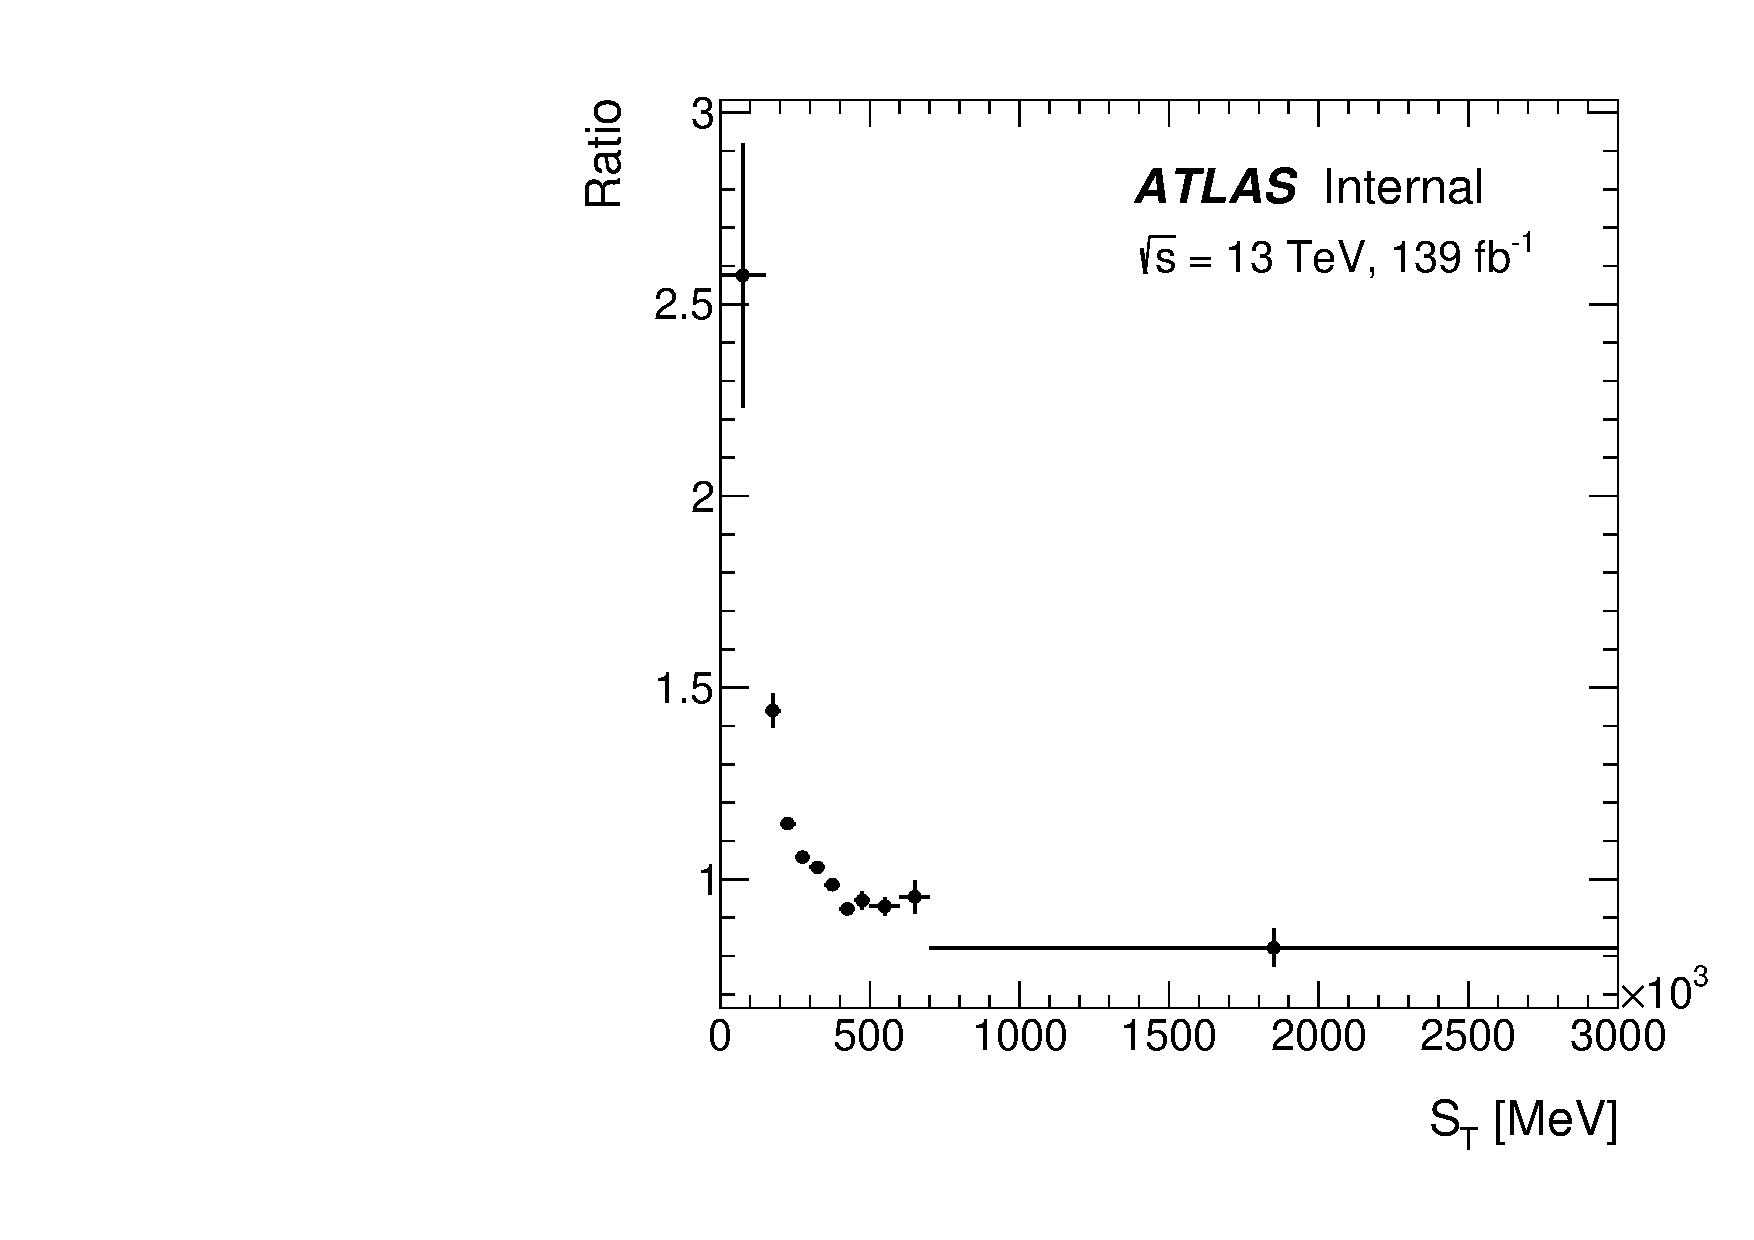
\includegraphics[width=.32\textwidth]{DiHiggs/plots/TtbarReweighting/wt1d_st_fr_os_2.pdf} }
  \subfloat[$N_{\text{jets}} = 3$] { 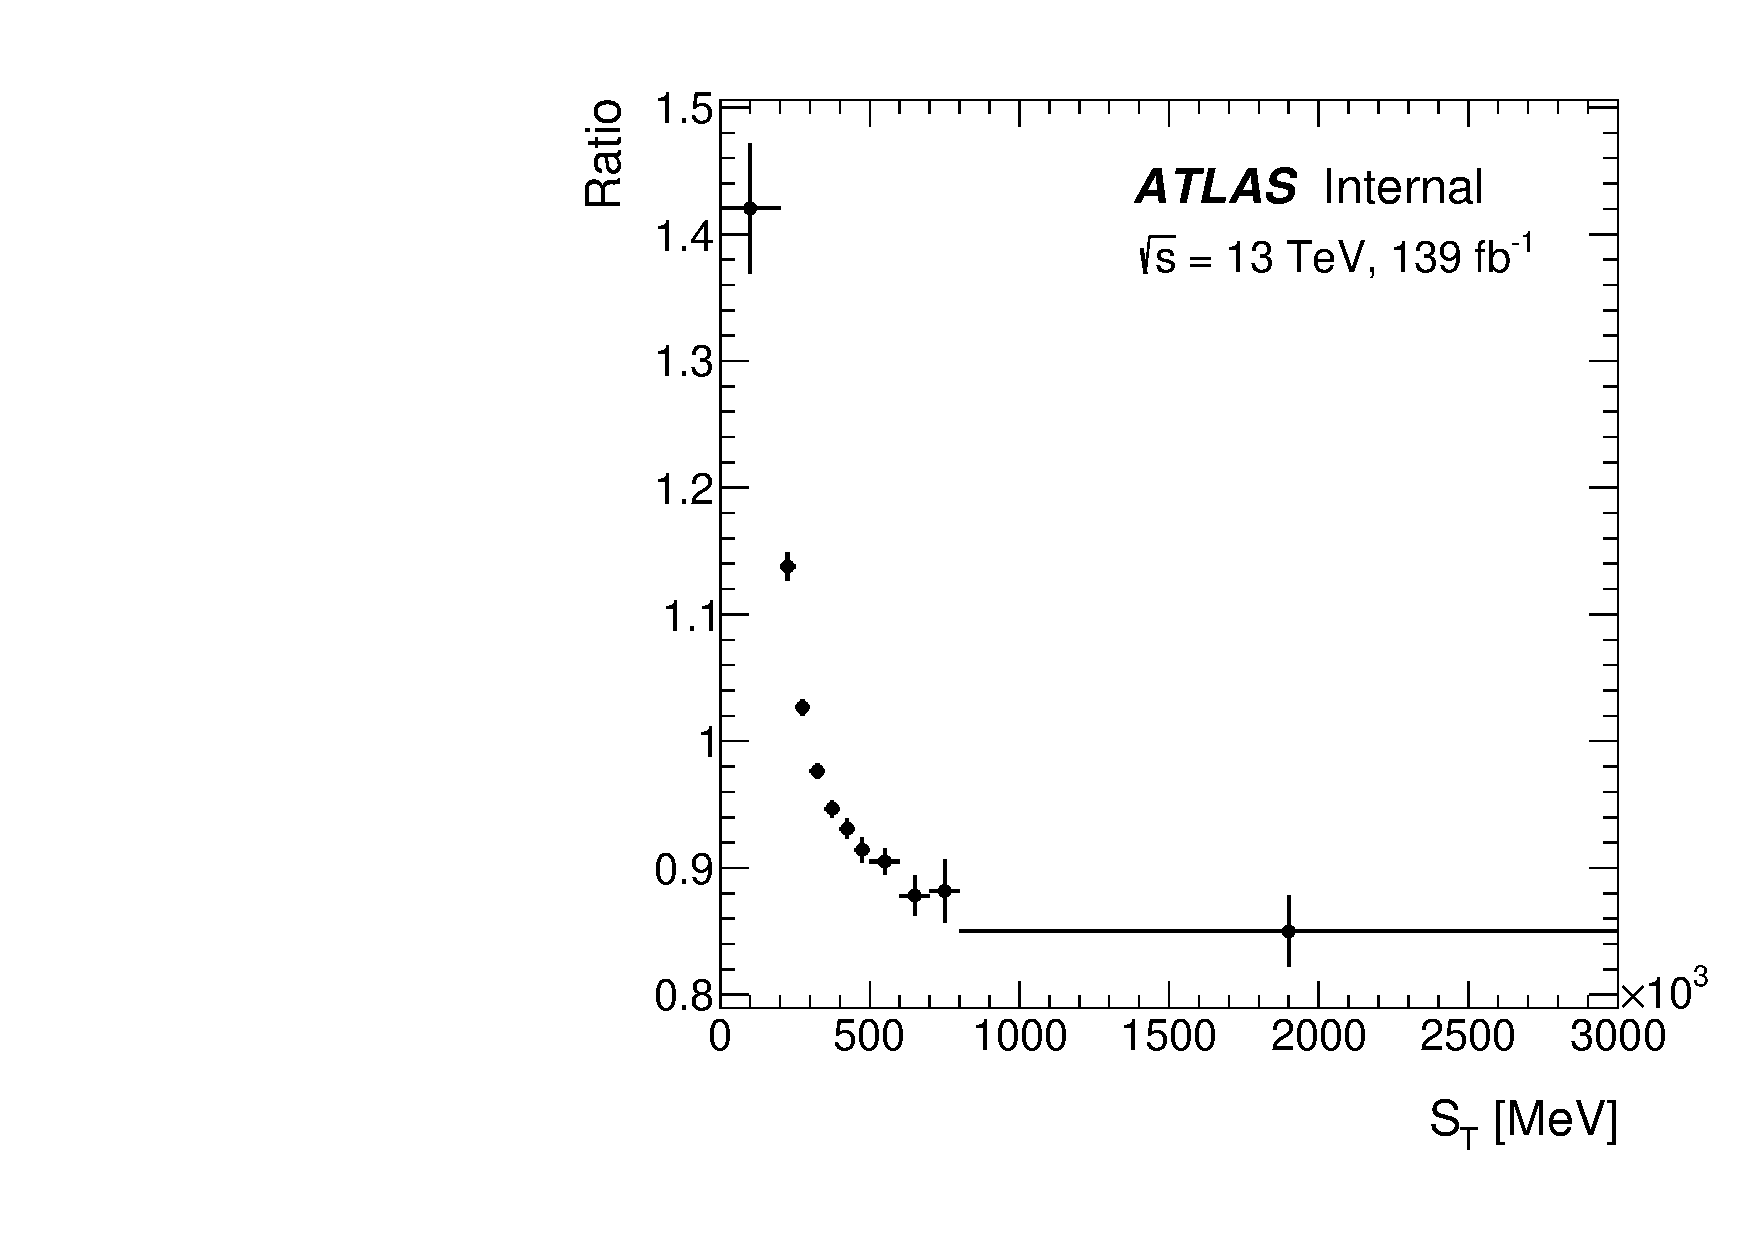
\includegraphics[width=.32\textwidth]{DiHiggs/plots/TtbarReweighting/wt1d_st_fr_os_3.pdf} }
  \subfloat[$N_{\text{jets}} = 4$] { 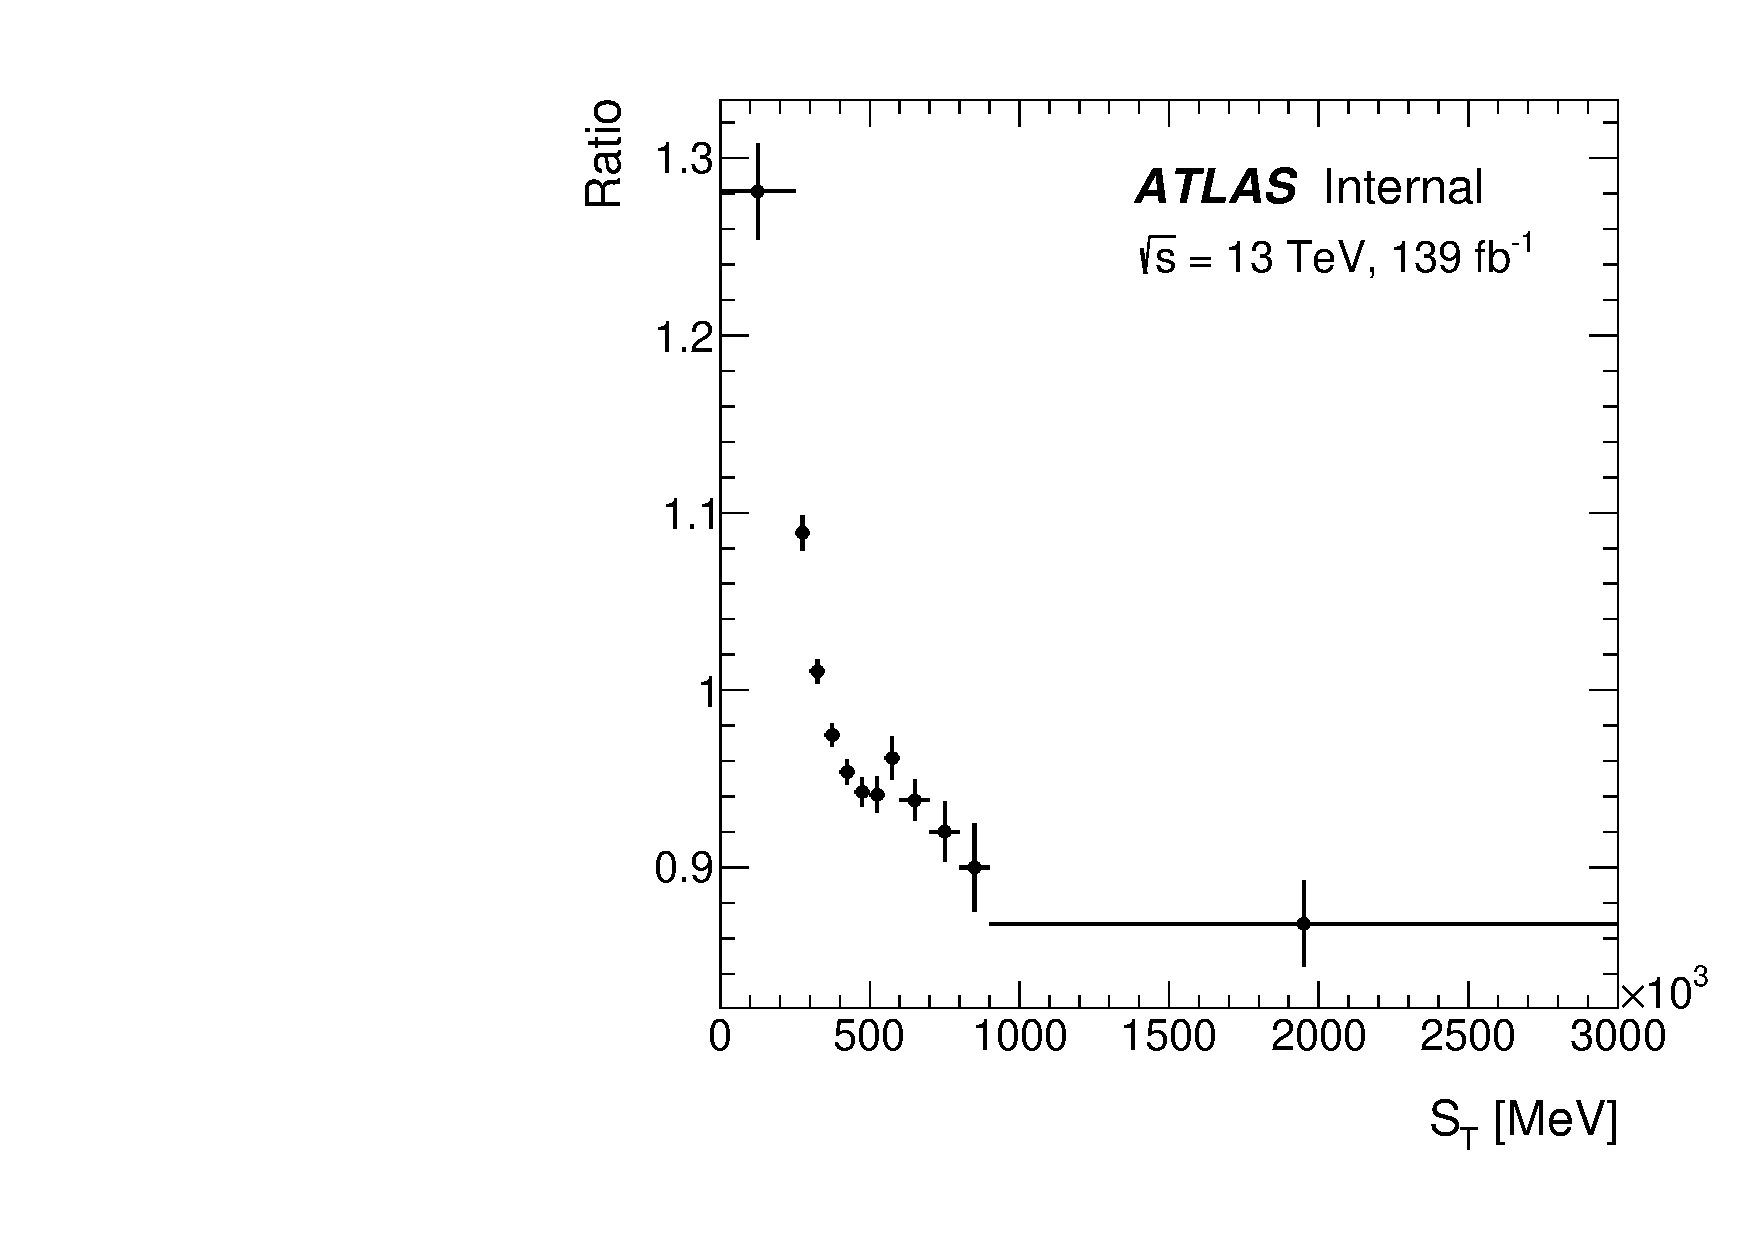
\includegraphics[width=.32\textwidth]{DiHiggs/plots/TtbarReweighting/wt1d_st_fr_os_4.pdf} } \\
  \subfloat[$N_{\text{jets}} = 5$] { 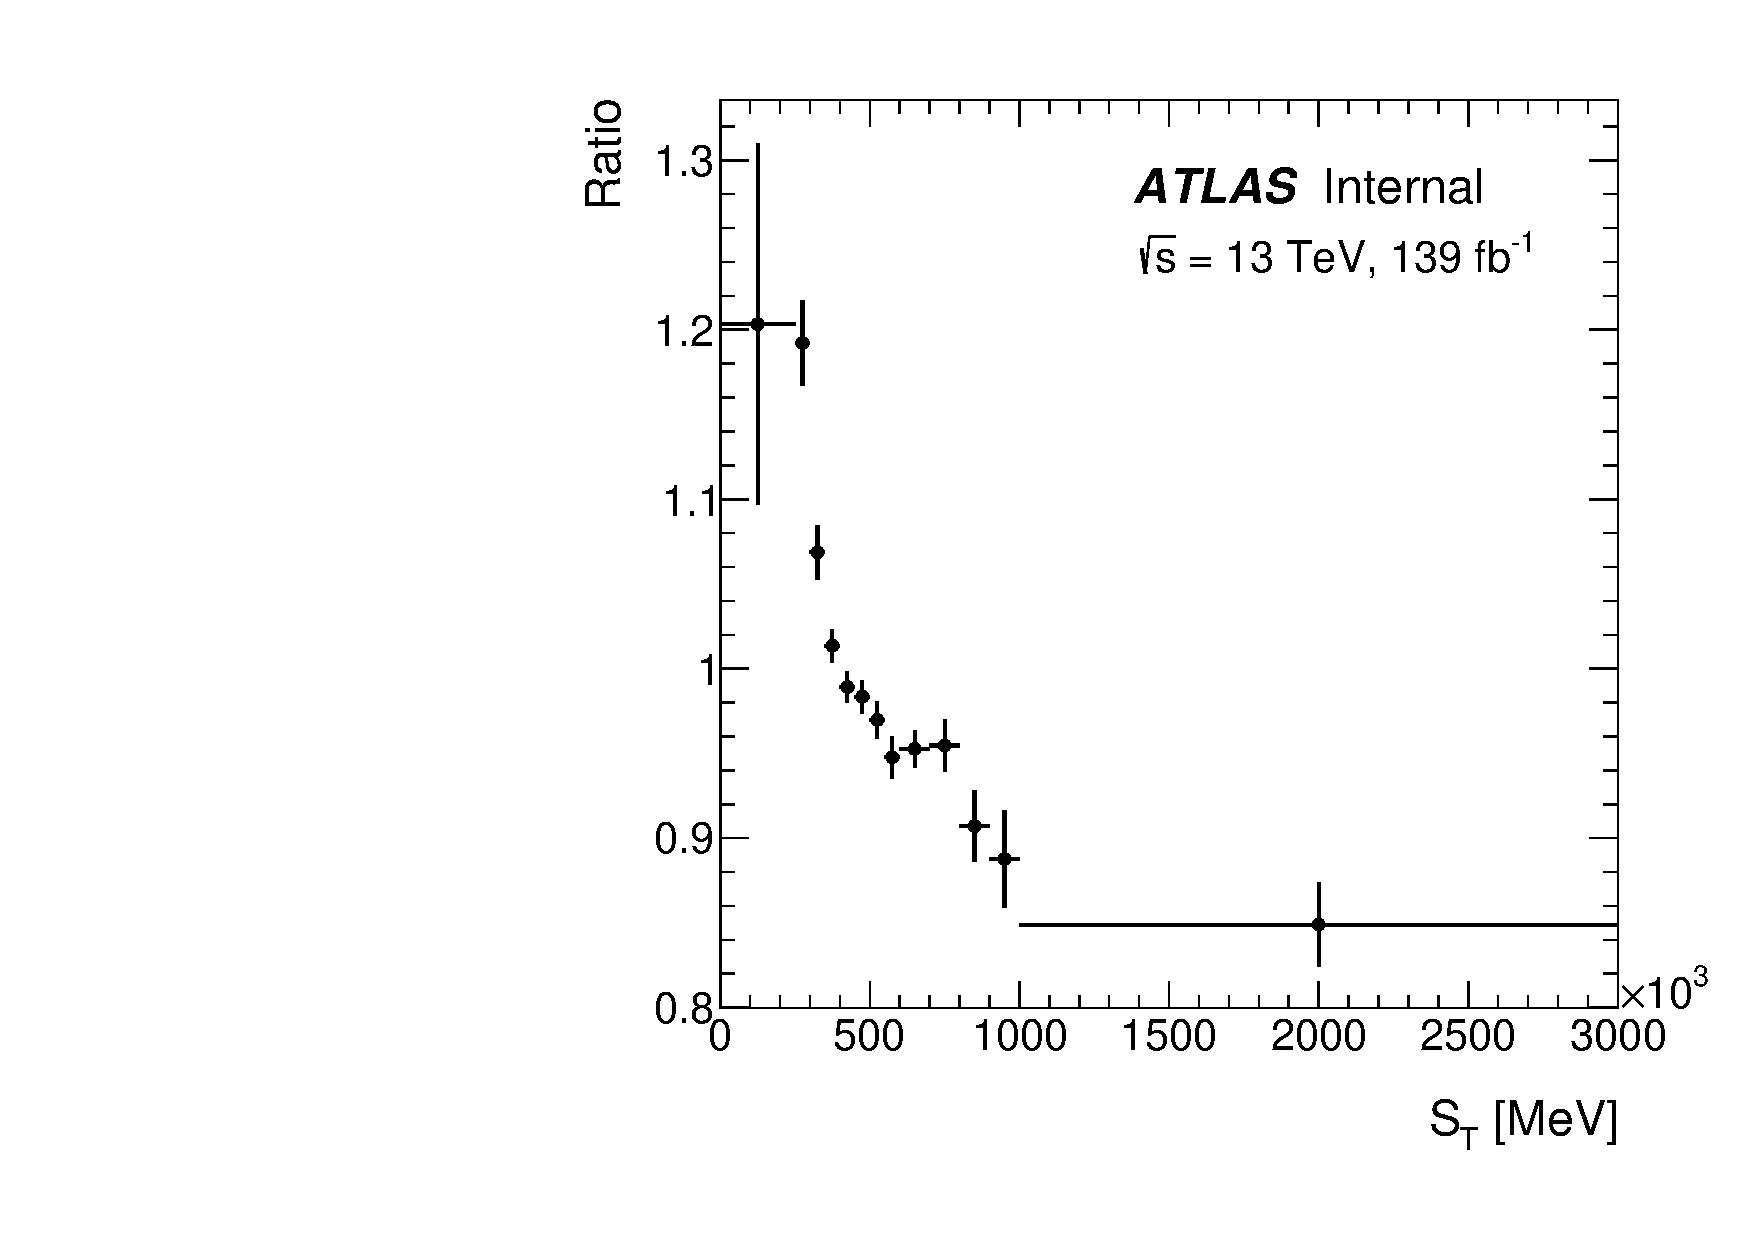
\includegraphics[width=.32\textwidth]{DiHiggs/plots/TtbarReweighting/wt1d_st_fr_os_5.pdf} }
  \subfloat[$N_{\text{jets}} = 6$] { 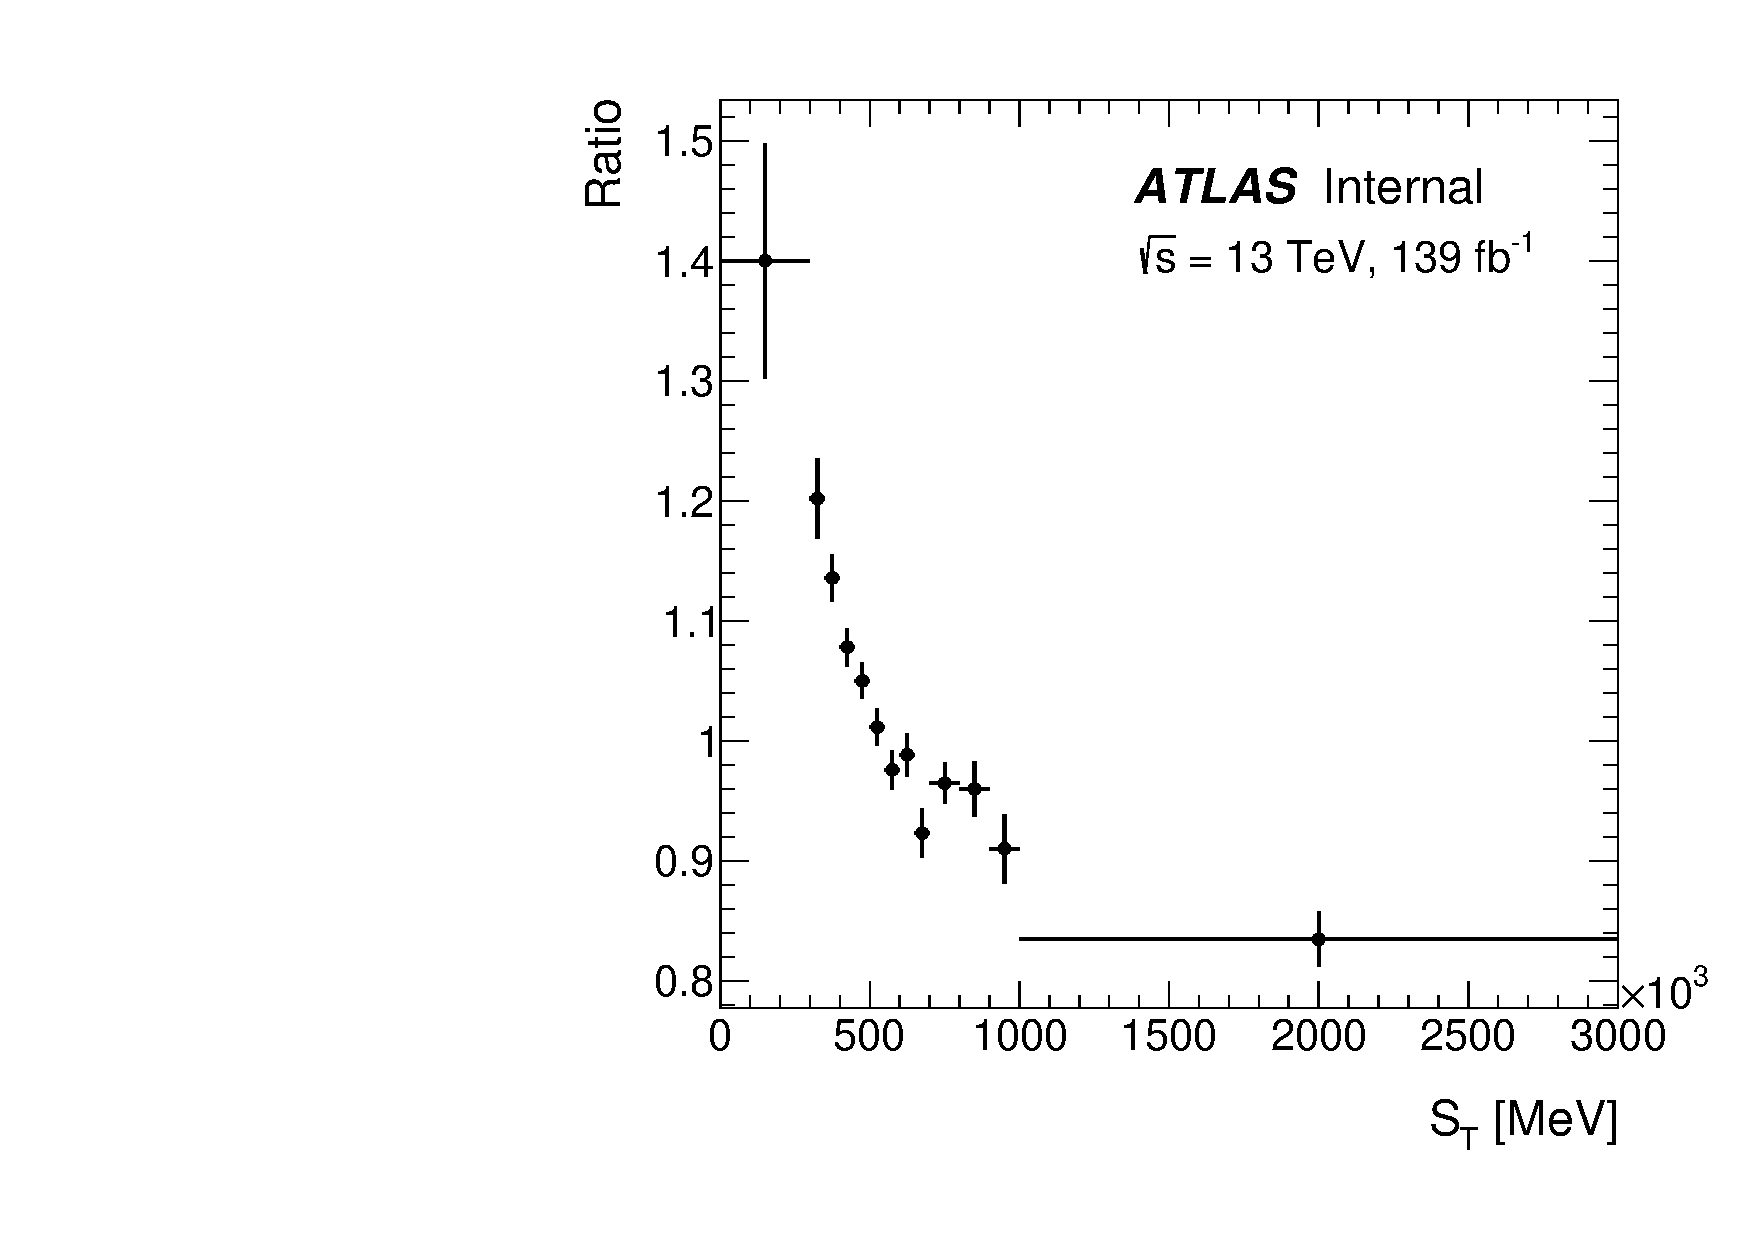
\includegraphics[width=.32\textwidth]{DiHiggs/plots/TtbarReweighting/wt1d_st_fr_os_6.pdf} }
  \subfloat[$N_{\text{jets}} = 7$] { 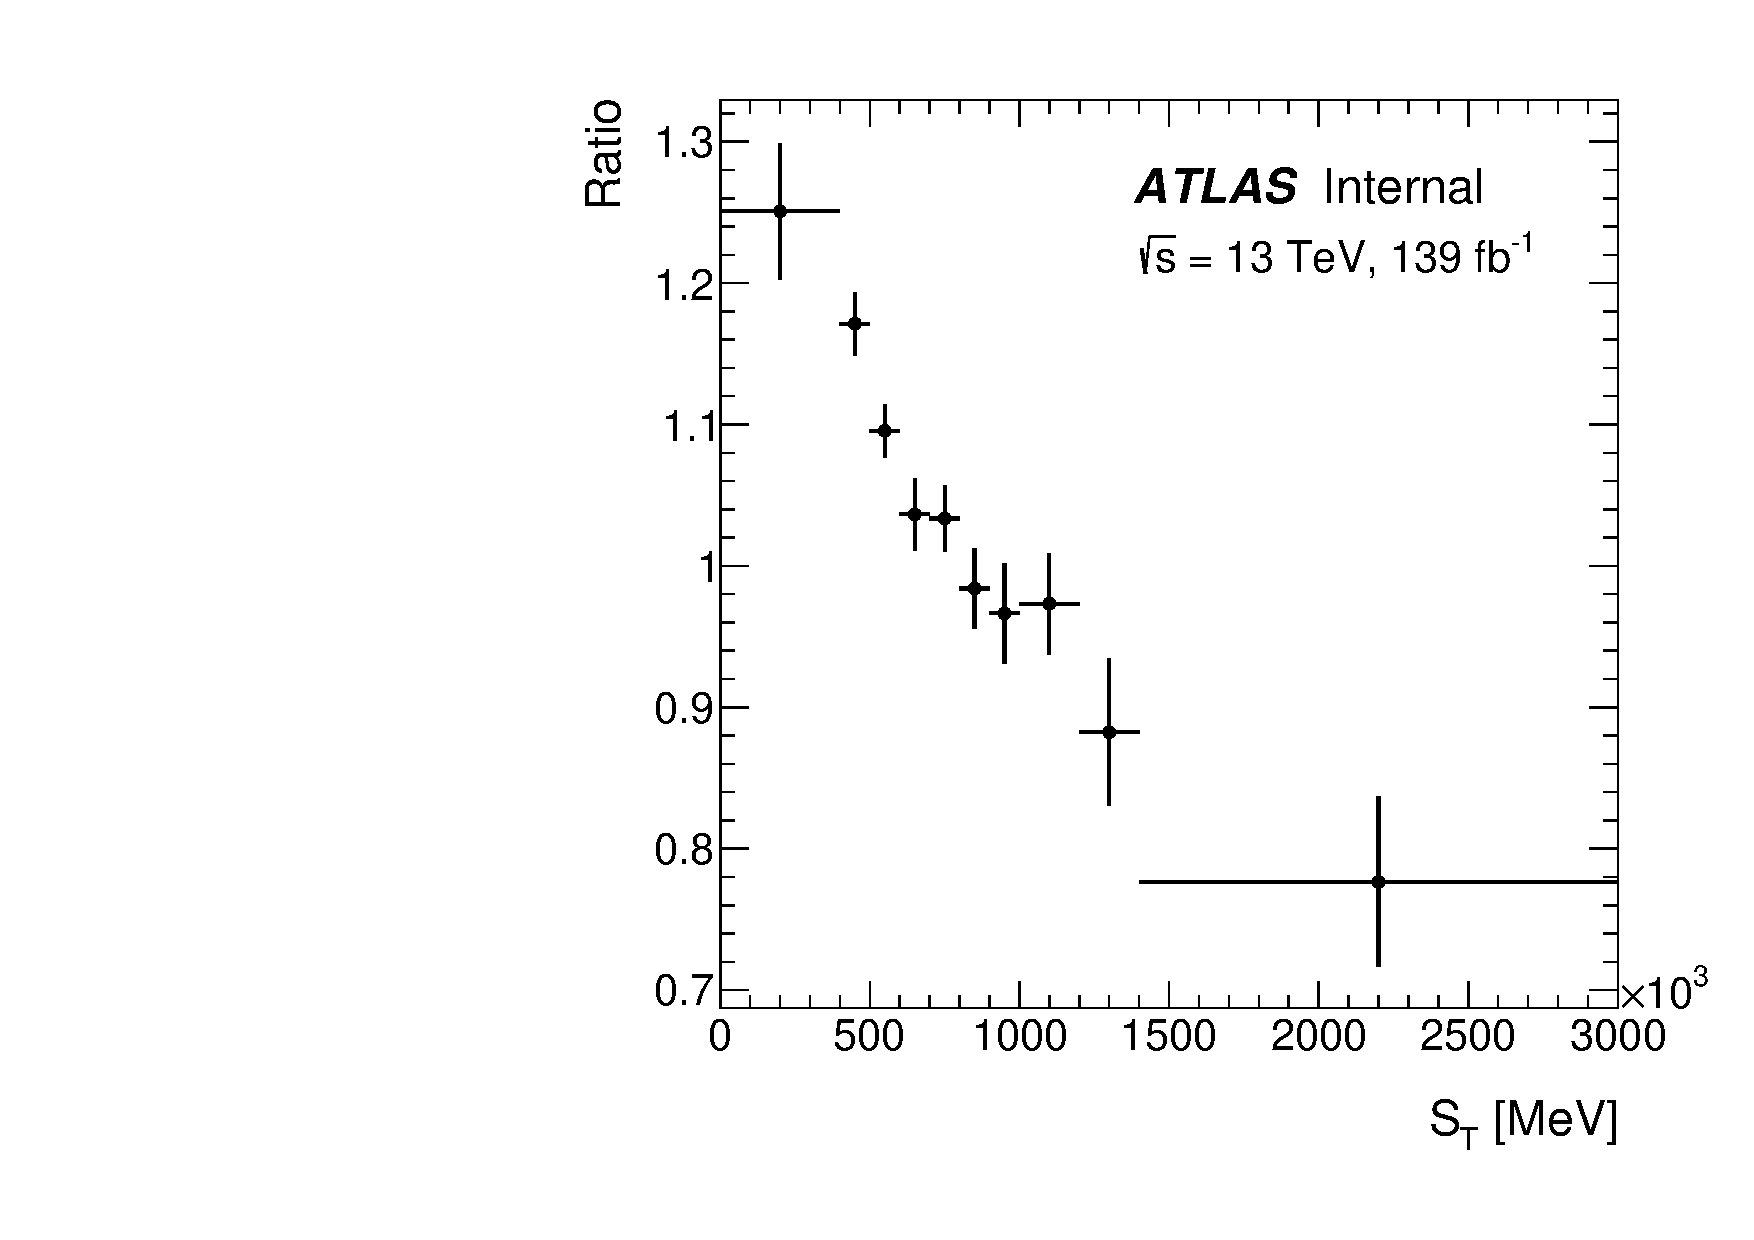
\includegraphics[width=.32\textwidth]{DiHiggs/plots/TtbarReweighting/wt1d_st_fr_os_7.pdf} } \\ 
  \subfloat[$N_{\text{jets}} = 8$] { 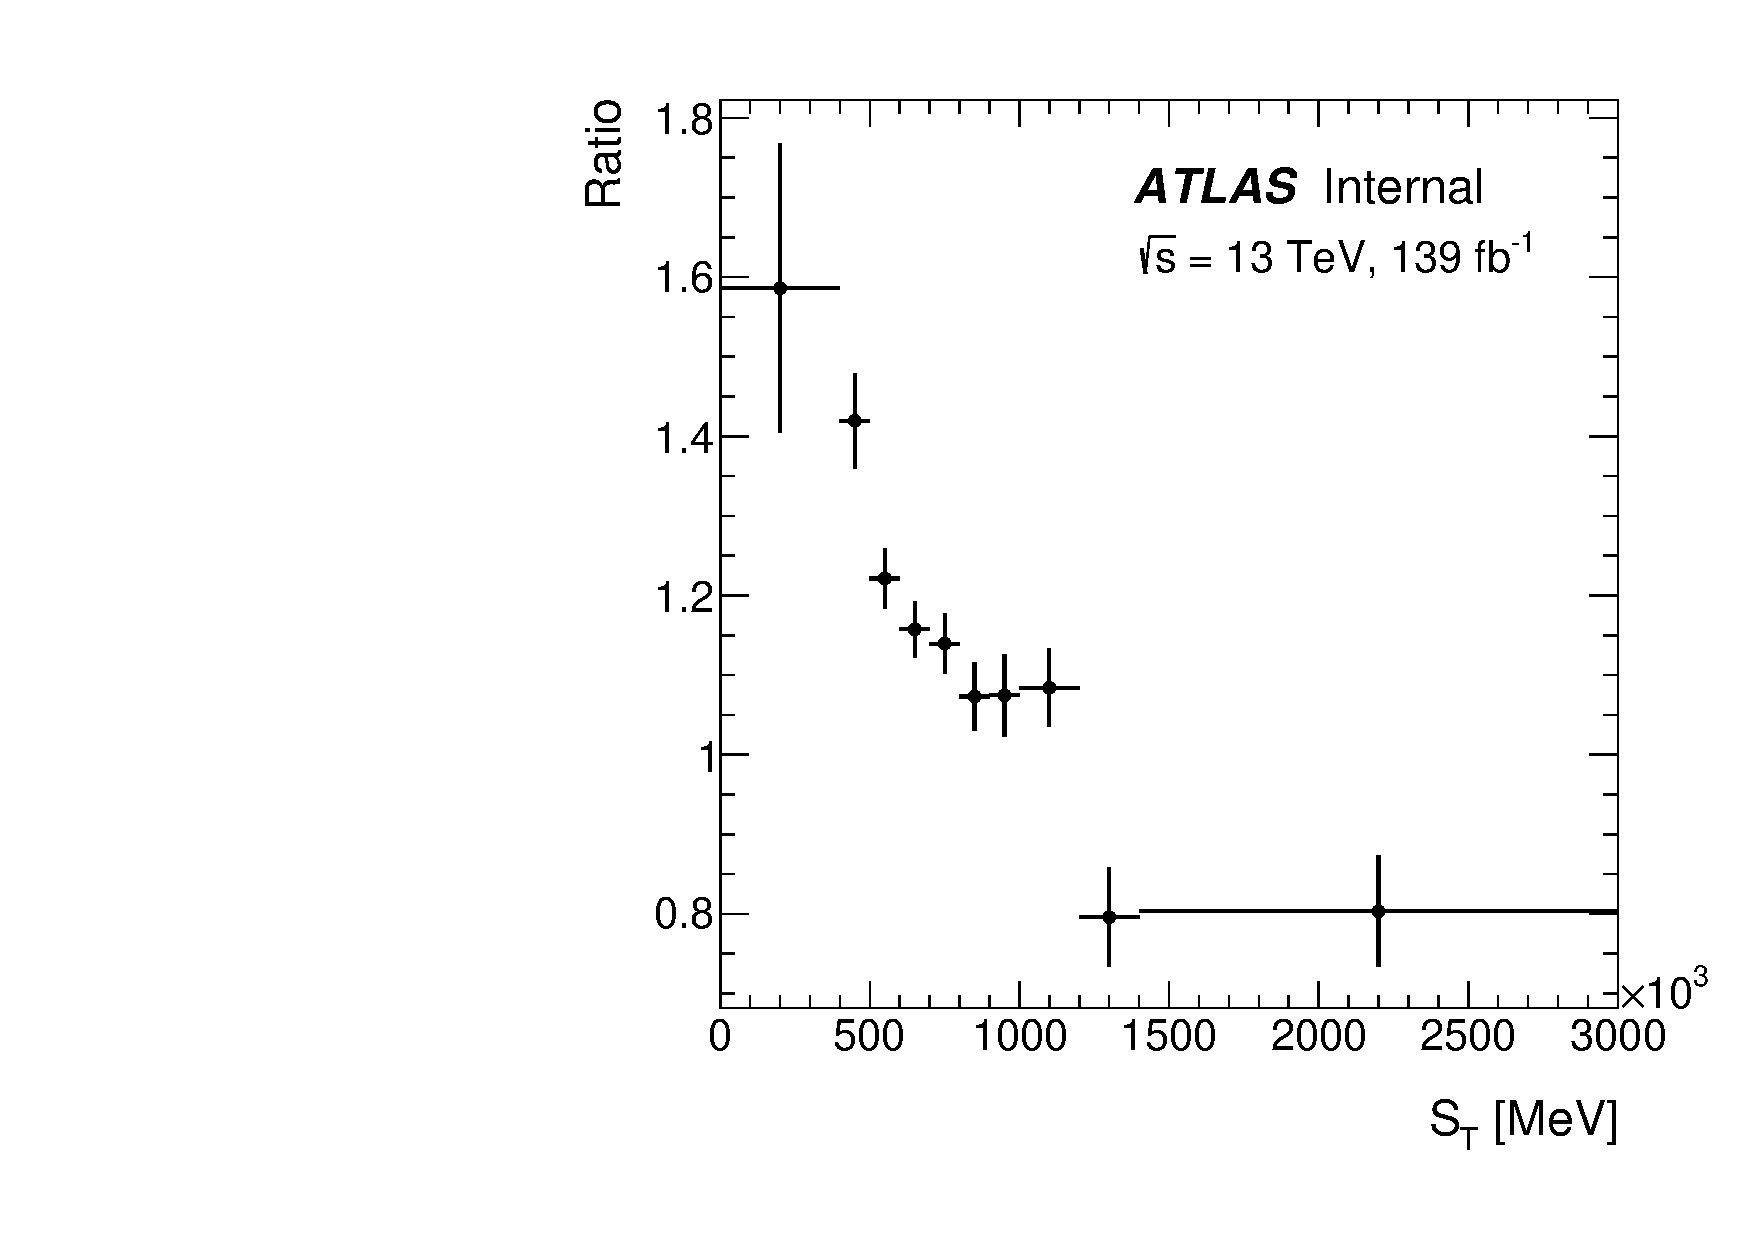
\includegraphics[width=.32\textwidth]{DiHiggs/plots/TtbarReweighting/wt1d_st_fr_os_8.pdf} }
  \subfloat[$N_{\text{jets}} = 9$] { 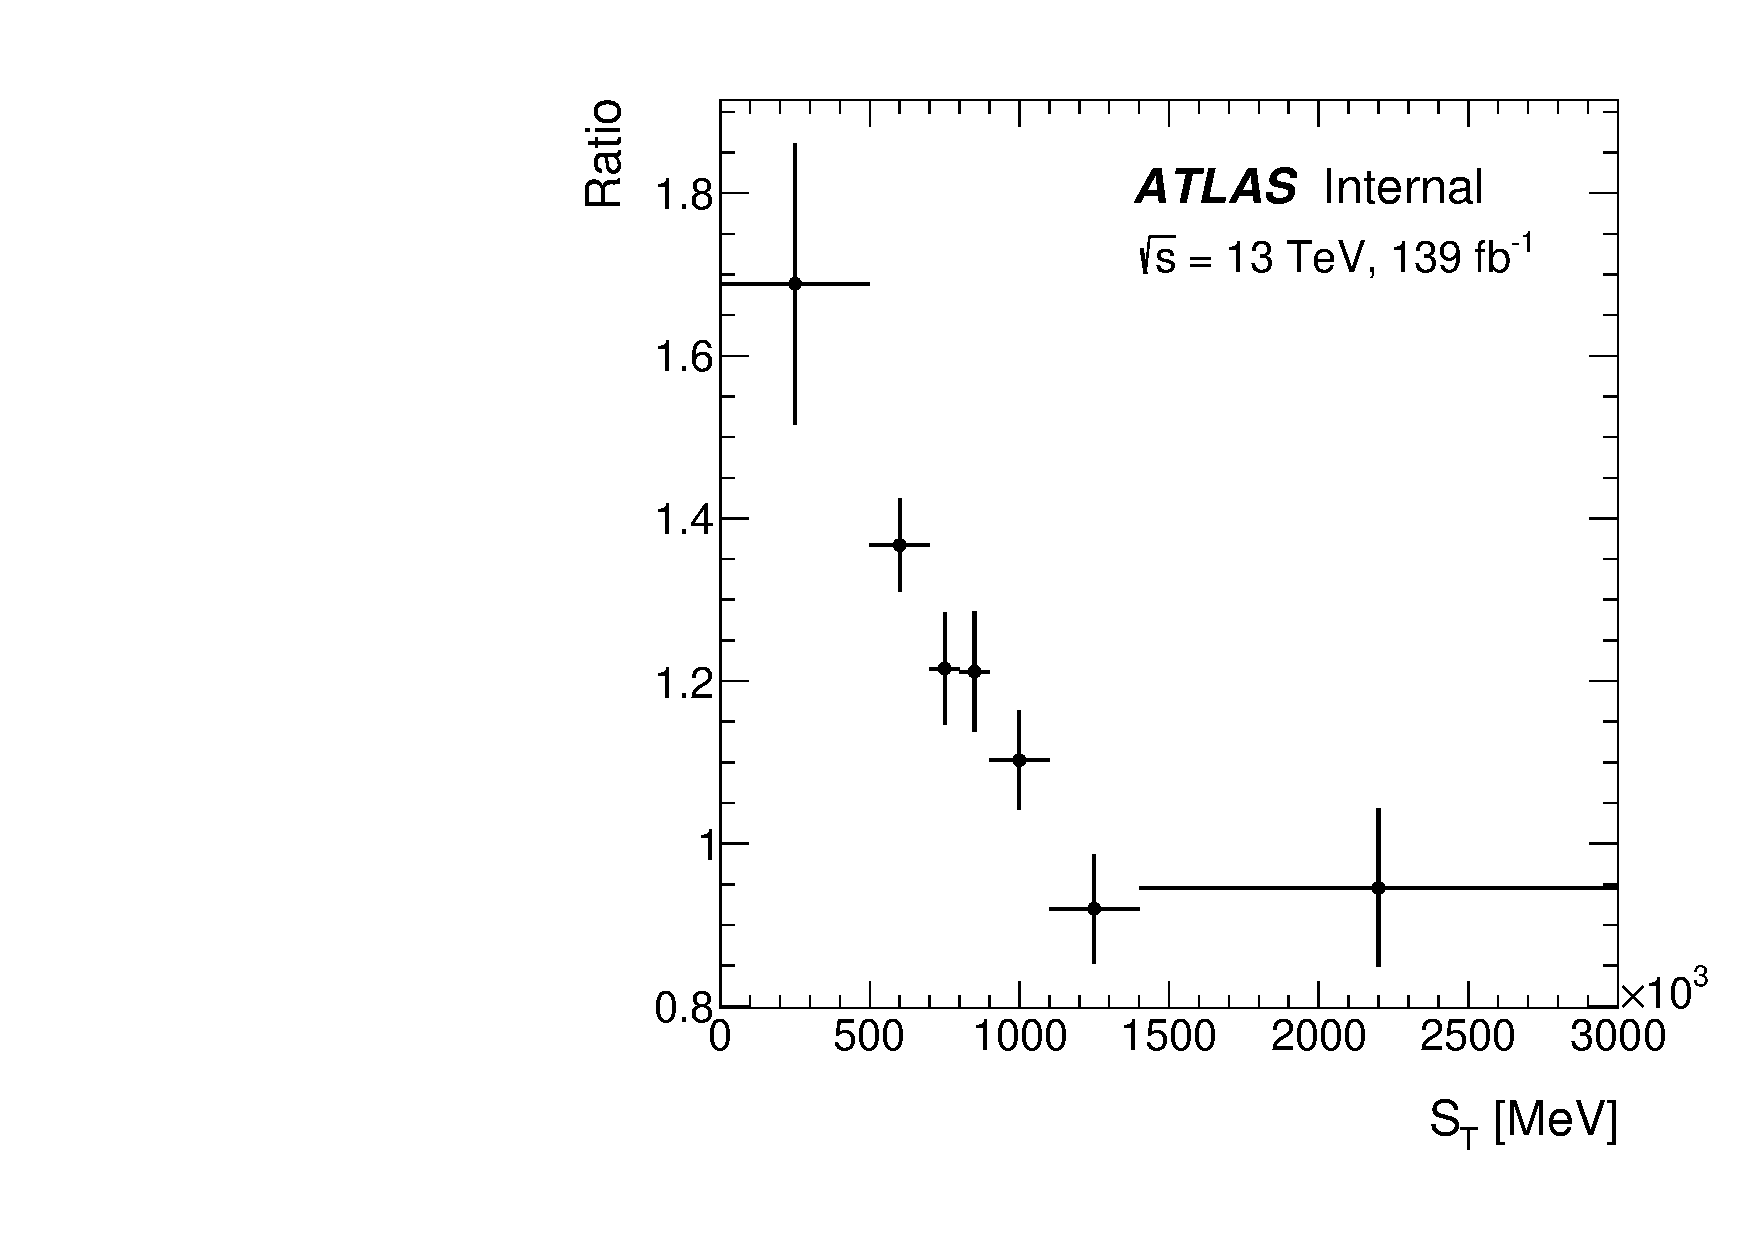
\includegraphics[width=.32\textwidth]{DiHiggs/plots/TtbarReweighting/wt1d_st_fr_os_9.pdf} }
  \subfloat[$N_{\text{jets}} \le 10$] { 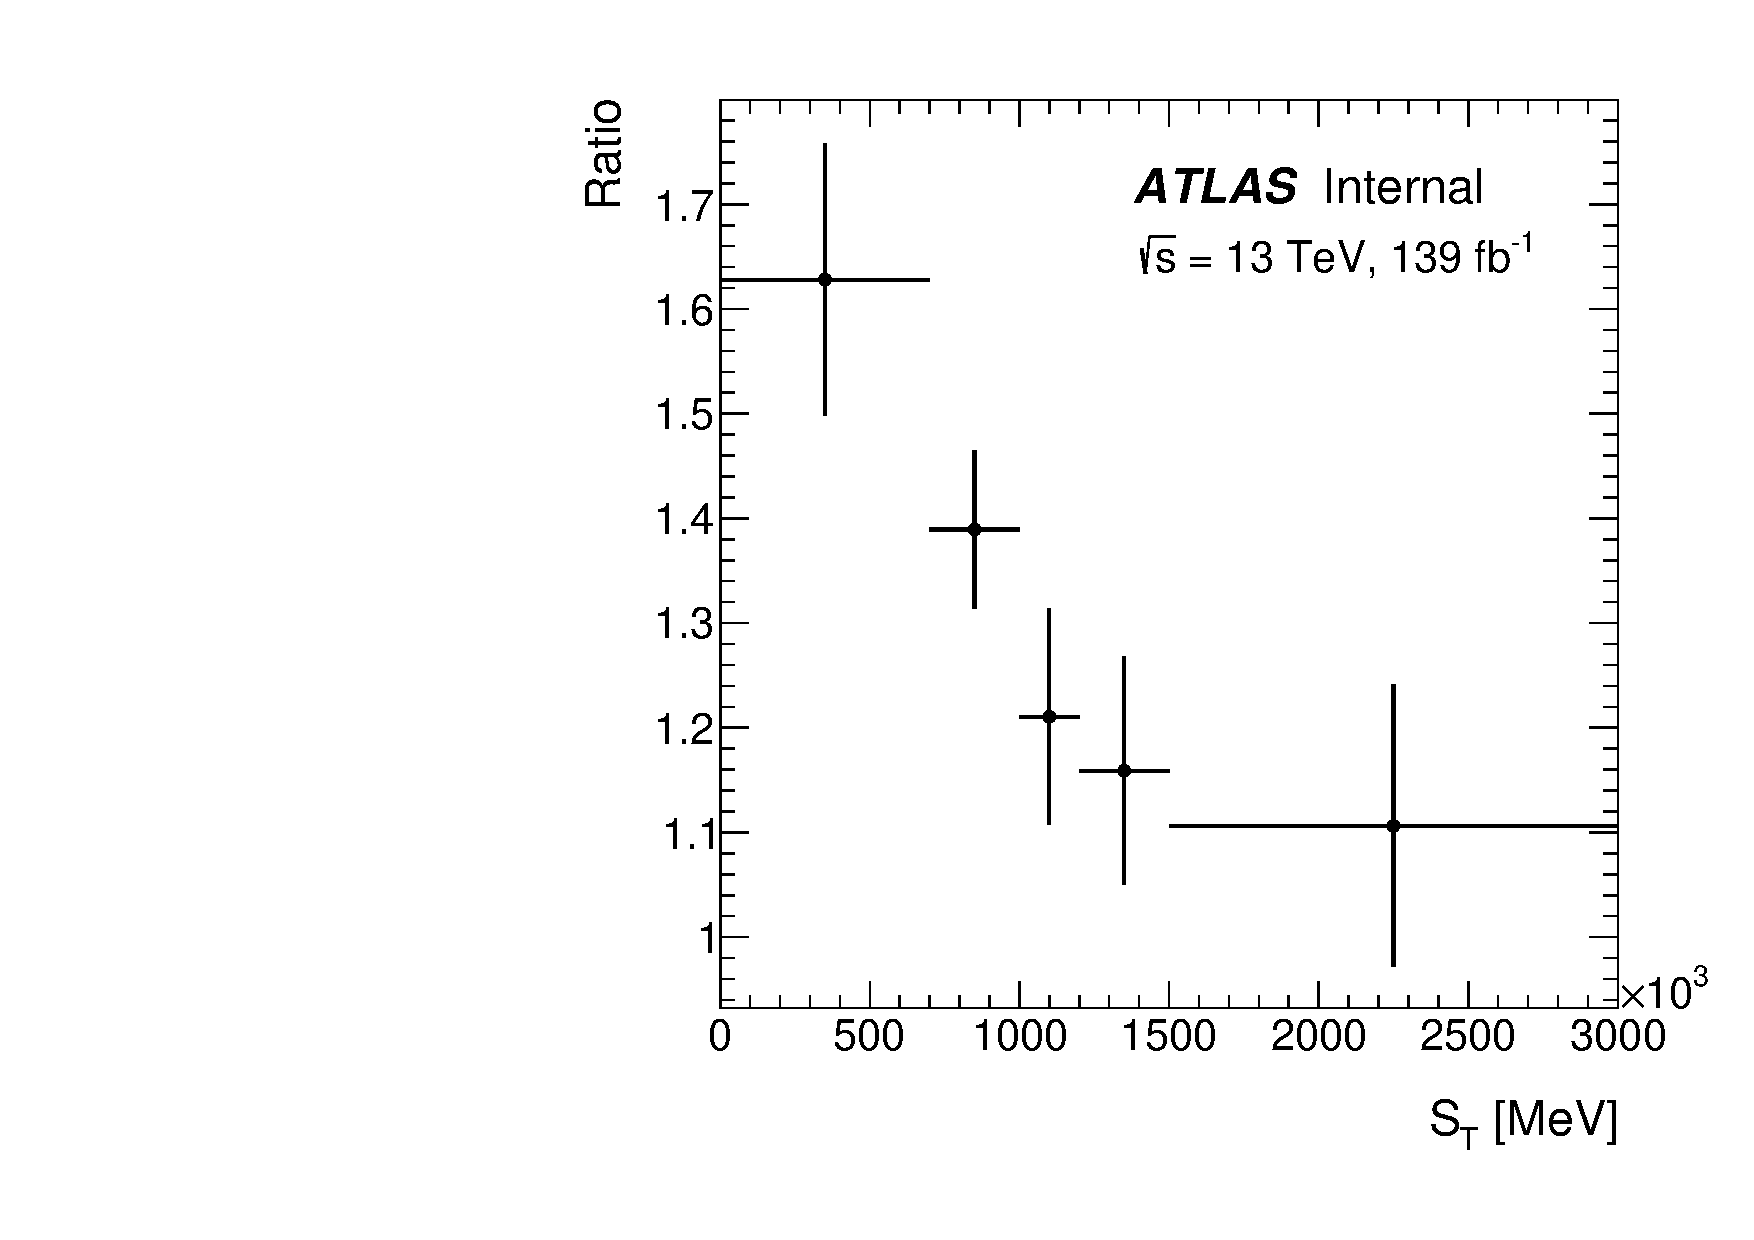
\includegraphics[width=.32\textwidth]{DiHiggs/plots/TtbarReweighting/wt1d_st_fr_os_10.pdf} }
  \caption{The \ttbar shape correction scale factor as functions of $H_{\text{T}}$ in different $N_{\text{jets}}$. 
  The error bars are calculated from the statistical uncertainties of data and simulated samples.
  Figures reproduced from analysis internal notes.}
  \label{fig:ttbarReweighting_parametrisations}
\end{figure}







\section{Additional material for MVA signal extraction}
\label{sec:appendix:mva}

\begin{figure}
    \centering
    \subfloat[]{\includegraphics[width=.45\textwidth]{diHiggs/plots/MVA/LephadOvertrainingPlots_10May21/SLT/NR/All/PNN.pdf}}\quad
    \subfloat[]{\includegraphics[width=.45\textwidth]{diHiggs/plots/MVA/LephadOvertrainingPlots_10May21/SLT/300/All/PNN300.pdf}}\quad\\
    \subfloat[]{\includegraphics[width=.45\textwidth]{diHiggs/plots/MVA/LephadOvertrainingPlots_10May21/SLT/500/All/PNN500.pdf}}\quad
    \subfloat[]{\includegraphics[width=.45\textwidth]{diHiggs/plots/MVA/LephadOvertrainingPlots_10May21/SLT/1000/All/PNN1000.pdf}}\quad
    \caption{(P)NN output distributions for (a) non-resonant signal, 
    and target signal masses of (b) 300~GeV, (c) 500~GeV, 
    and (d) 1000~GeV obtained evaluating the MVA with even-odd 
    events crossing or evaluating the MVA on the training datasets for the SLT category. 
    The ``OT'' histograms refer to the ``OverTraining'' check in 
    which the (P)NN is applied to the same data on which it was trained, 
    the other histograms are obtained evaluating the MVA with even-odd event crossing.
    Images reproced from analysis internal notes.}
    \label{fig:overfittingtestSLT}
  \end{figure}
  
  \begin{figure}
    \centering
    \subfloat[]{\includegraphics[width=.45\textwidth]{diHiggs/plots/MVA/LephadOvertrainingPlots_10May21/LTT/NR/All/PNN.pdf}}\quad
    \subfloat[]{\includegraphics[width=.45\textwidth]{diHiggs/plots/MVA/LephadOvertrainingPlots_10May21/LTT/300/All/PNN300.pdf}}\quad\\
    \subfloat[]{\includegraphics[width=.45\textwidth]{diHiggs/plots/MVA/LephadOvertrainingPlots_10May21/LTT/500/All/PNN500.pdf}}\quad
    \subfloat[]{\includegraphics[width=.45\textwidth]{diHiggs/plots/MVA/LephadOvertrainingPlots_10May21/LTT/1000/All/PNN1000.pdf}}\quad
    \caption{(P)NN output distributions for 
    (a) non-resonant signal, and target signal masses of 
    (b) 300~GeV, (c) 500~GeV, and (d) 1000~GeV obtained 
    evaluating the MVA with even-odd events crossing or 
    evaluating the MVA on the training datasets for the LTT category. 
    The ``OT'' histograms refer to the ``OverTraining'' check in which 
    the (P)NN is applied to the same data on which it was trained, 
    the other histograms are obtained evaluating the MVA with even-odd event crossing.
    Images reproced from analysis internal notes.}
    \label{fig:overfittingtestLTT}
  \end{figure}

  \begin{figure}
    \centering
    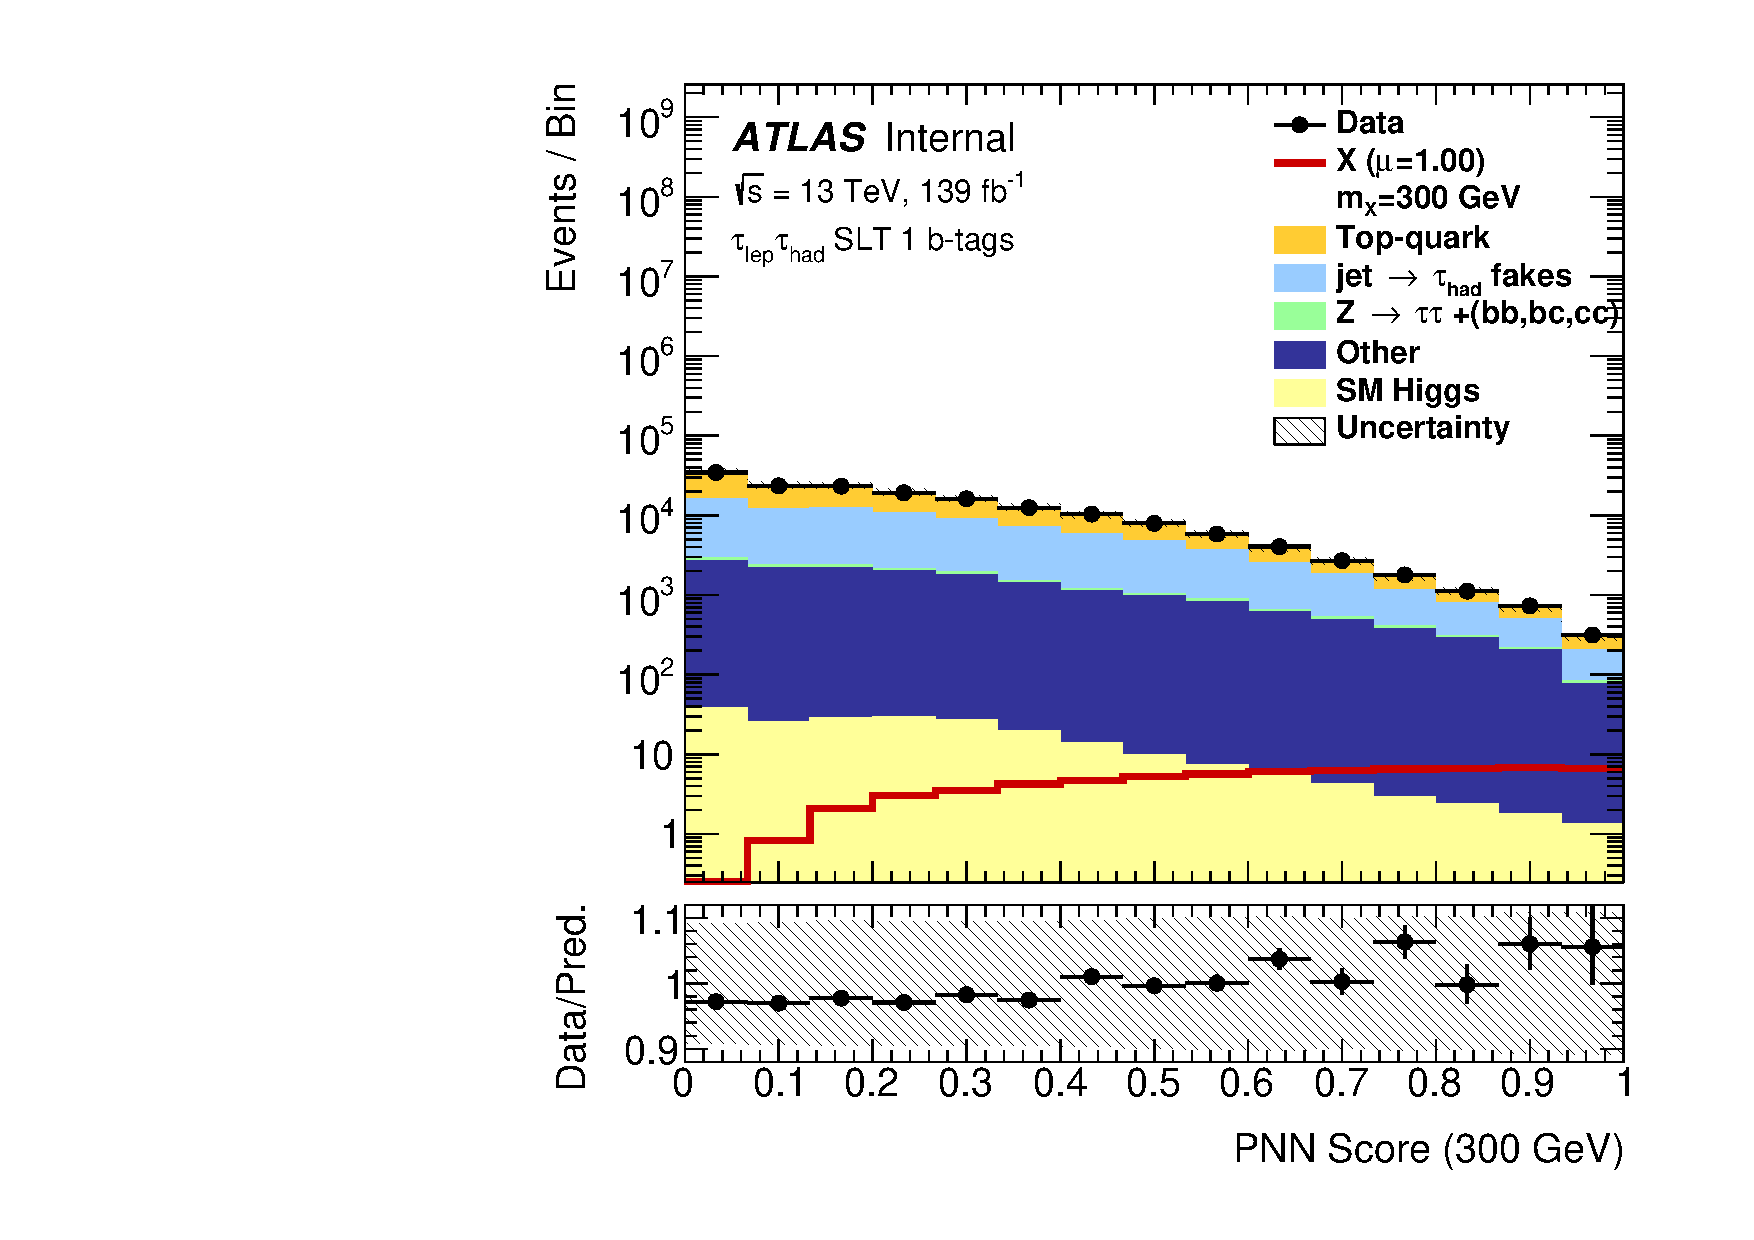
\includegraphics[width=.32\textwidth]{DiHiggs/plots/MVA/SLT/Region_BMin0_incJet1_dist300_J2_D2HDMPNN_T1_SpcTauLH_Y2015_LTT0_L1_Prefitlog.pdf}
    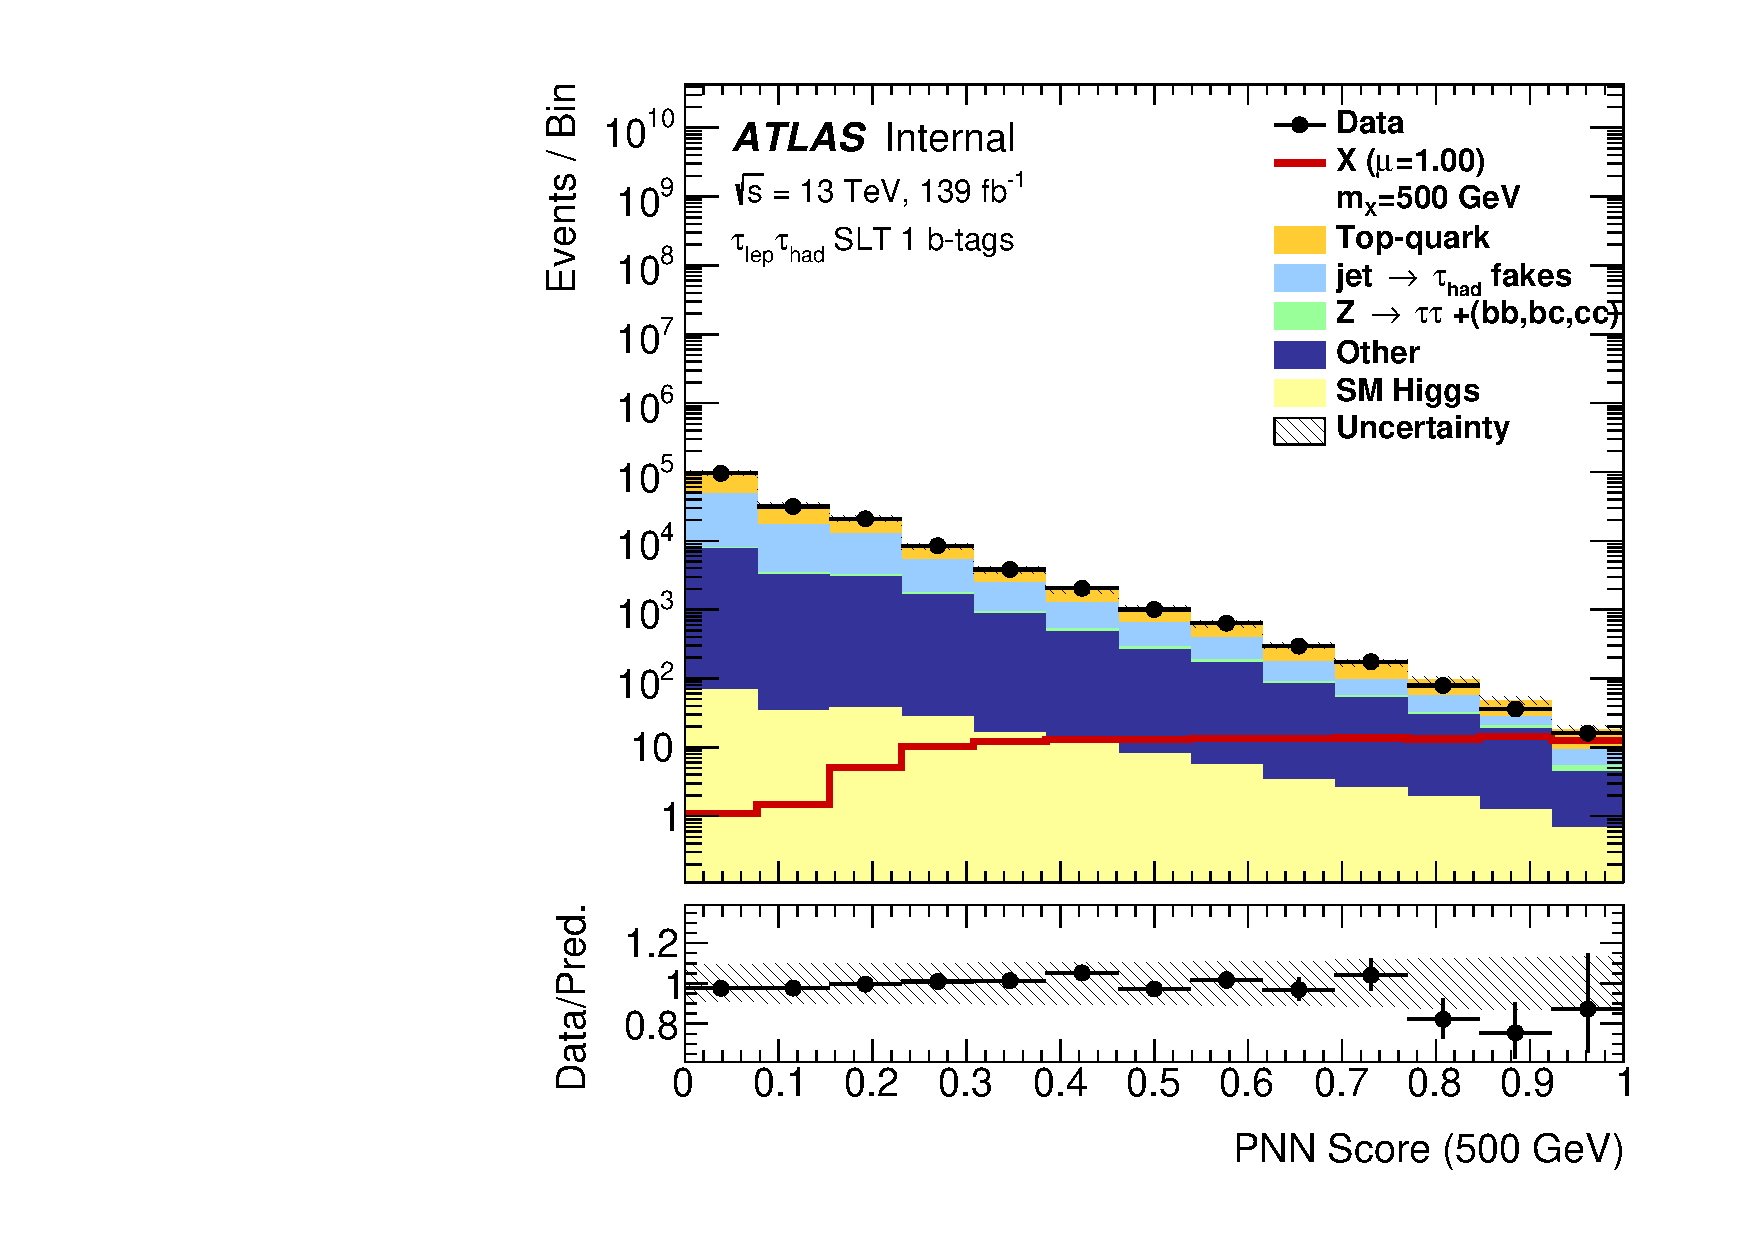
\includegraphics[width=.32\textwidth]{DiHiggs/plots/MVA/SLT/Region_BMin0_incJet1_dist500_J2_D2HDMPNN_T1_SpcTauLH_Y2015_LTT0_L1_Prefitlog.pdf}
    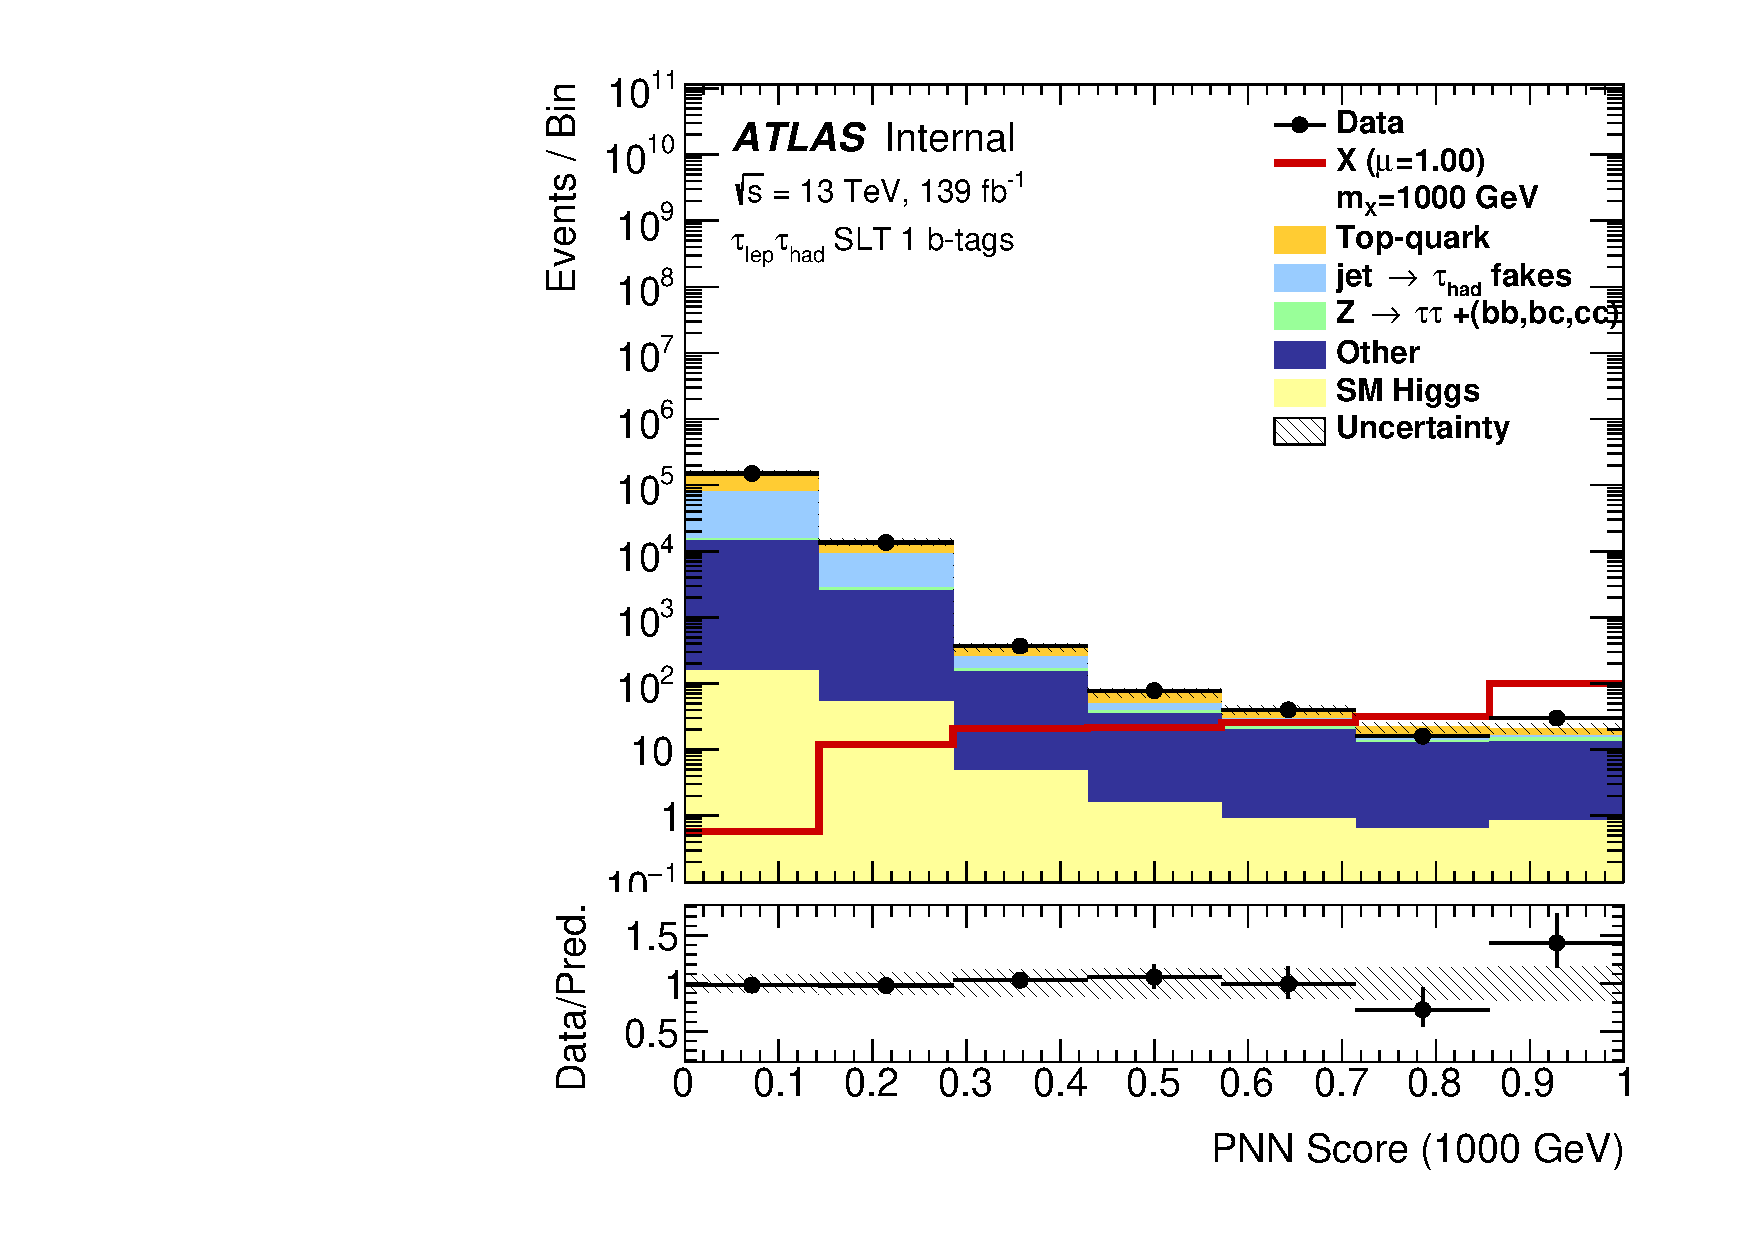
\includegraphics[width=.32\textwidth]{DiHiggs/plots/MVA/SLT/Region_BMin0_incJet1_dist1000_J2_D2HDMPNN_T1_SpcTauLH_Y2015_LTT0_L1_Prefitlog.pdf} \\
    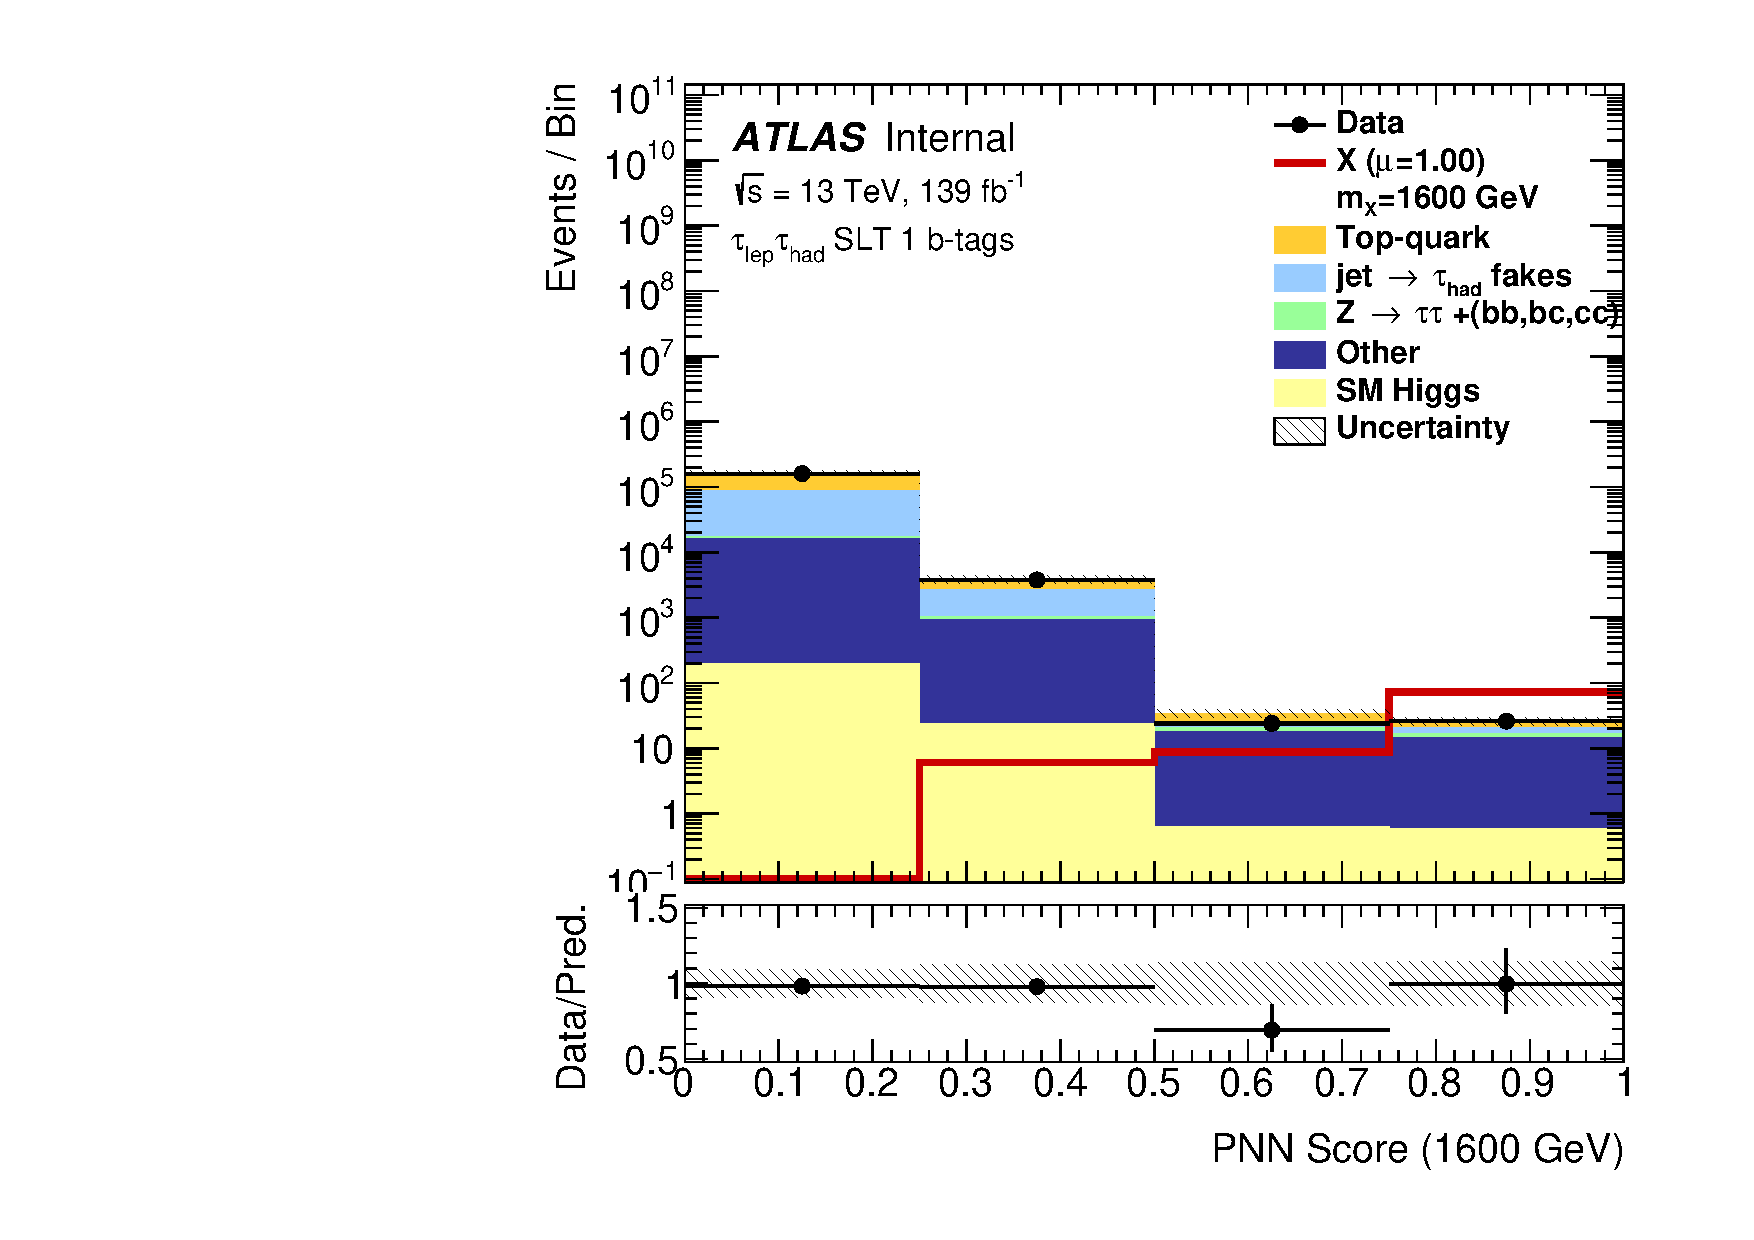
\includegraphics[width=.32\textwidth]{DiHiggs/plots/MVA/SLT/Region_BMin0_incJet1_dist1600_J2_D2HDMPNN_T1_SpcTauLH_Y2015_LTT0_L1_Prefitlog.pdf}
    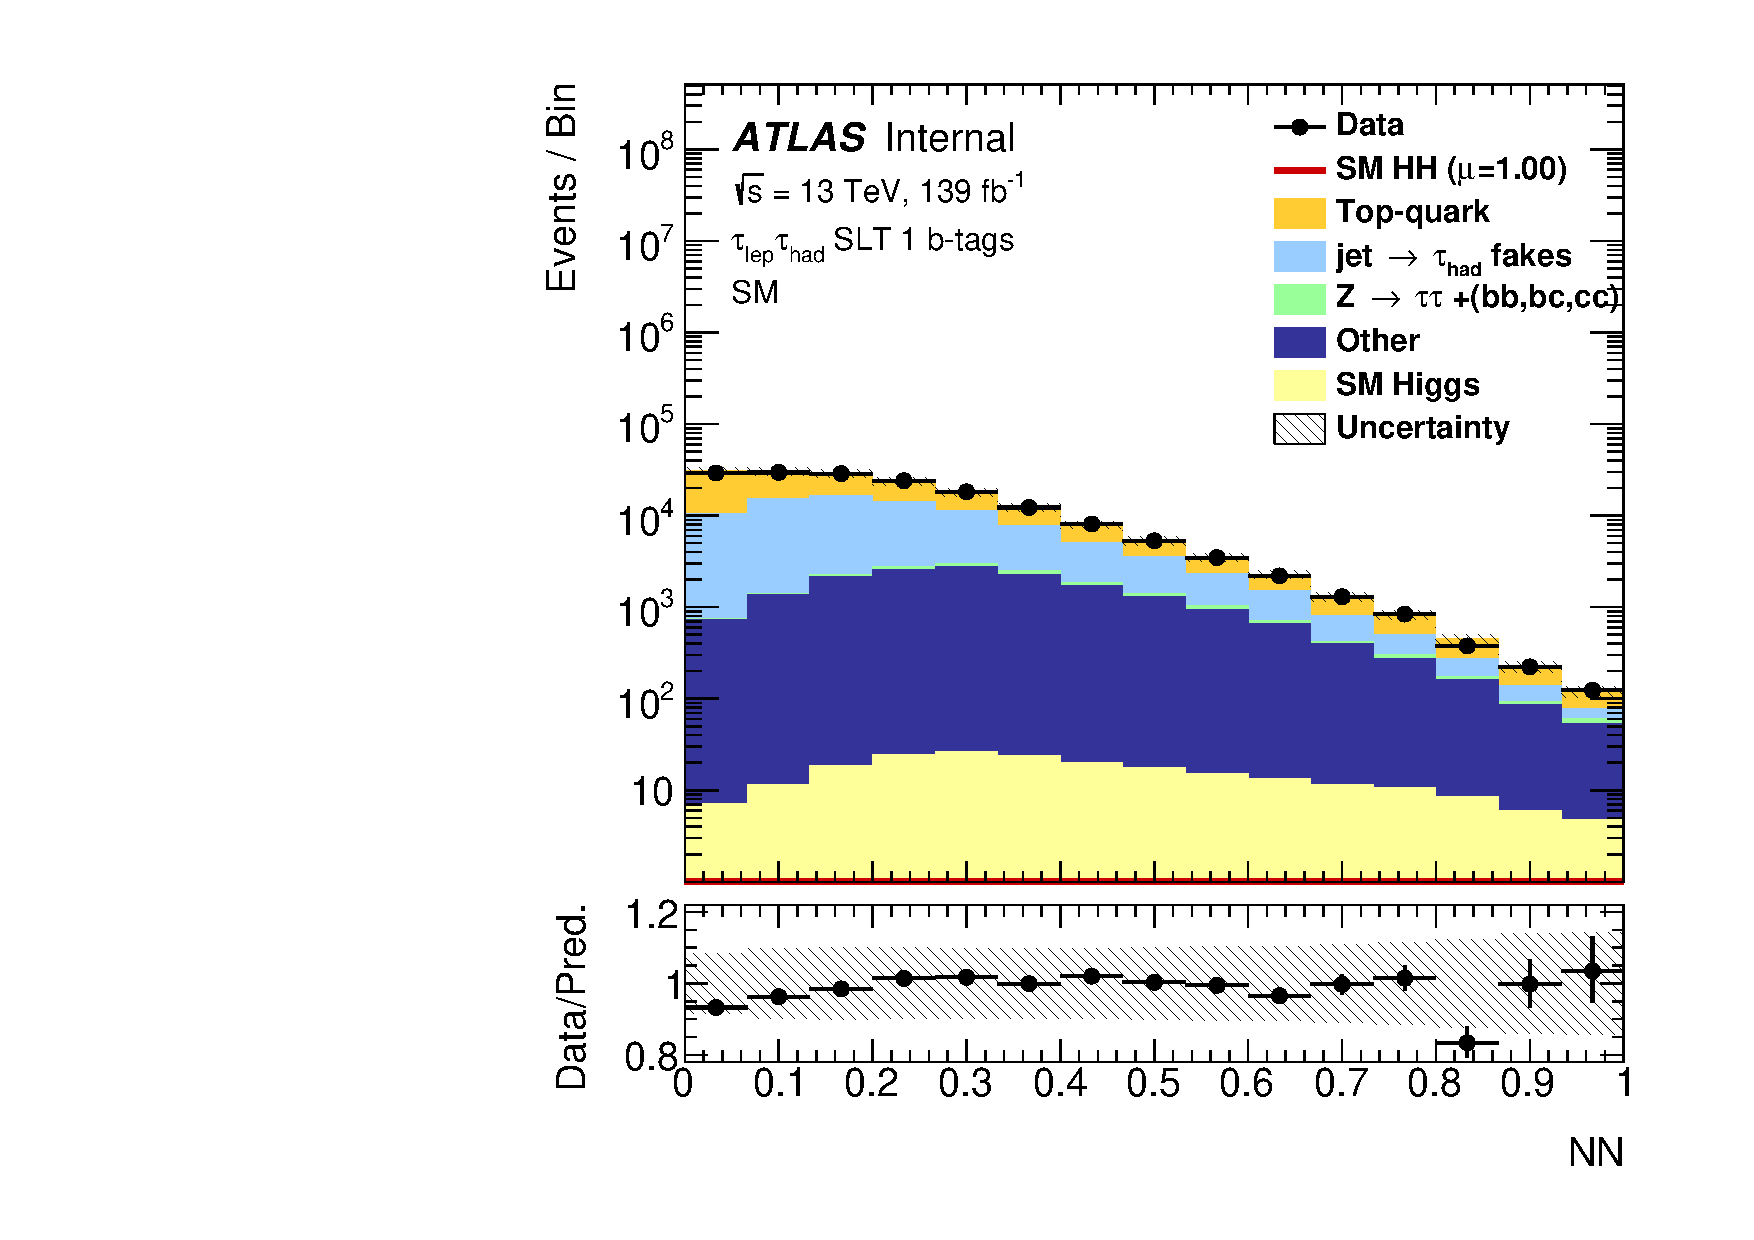
\includegraphics[width=.32\textwidth]{DiHiggs/plots/MVA/SLT/Region_BMin0_incJet1_distNN_J2_DSM_T1_SpcTauLH_Y2015_LTT0_L1_Prefitlog.pdf} \\
    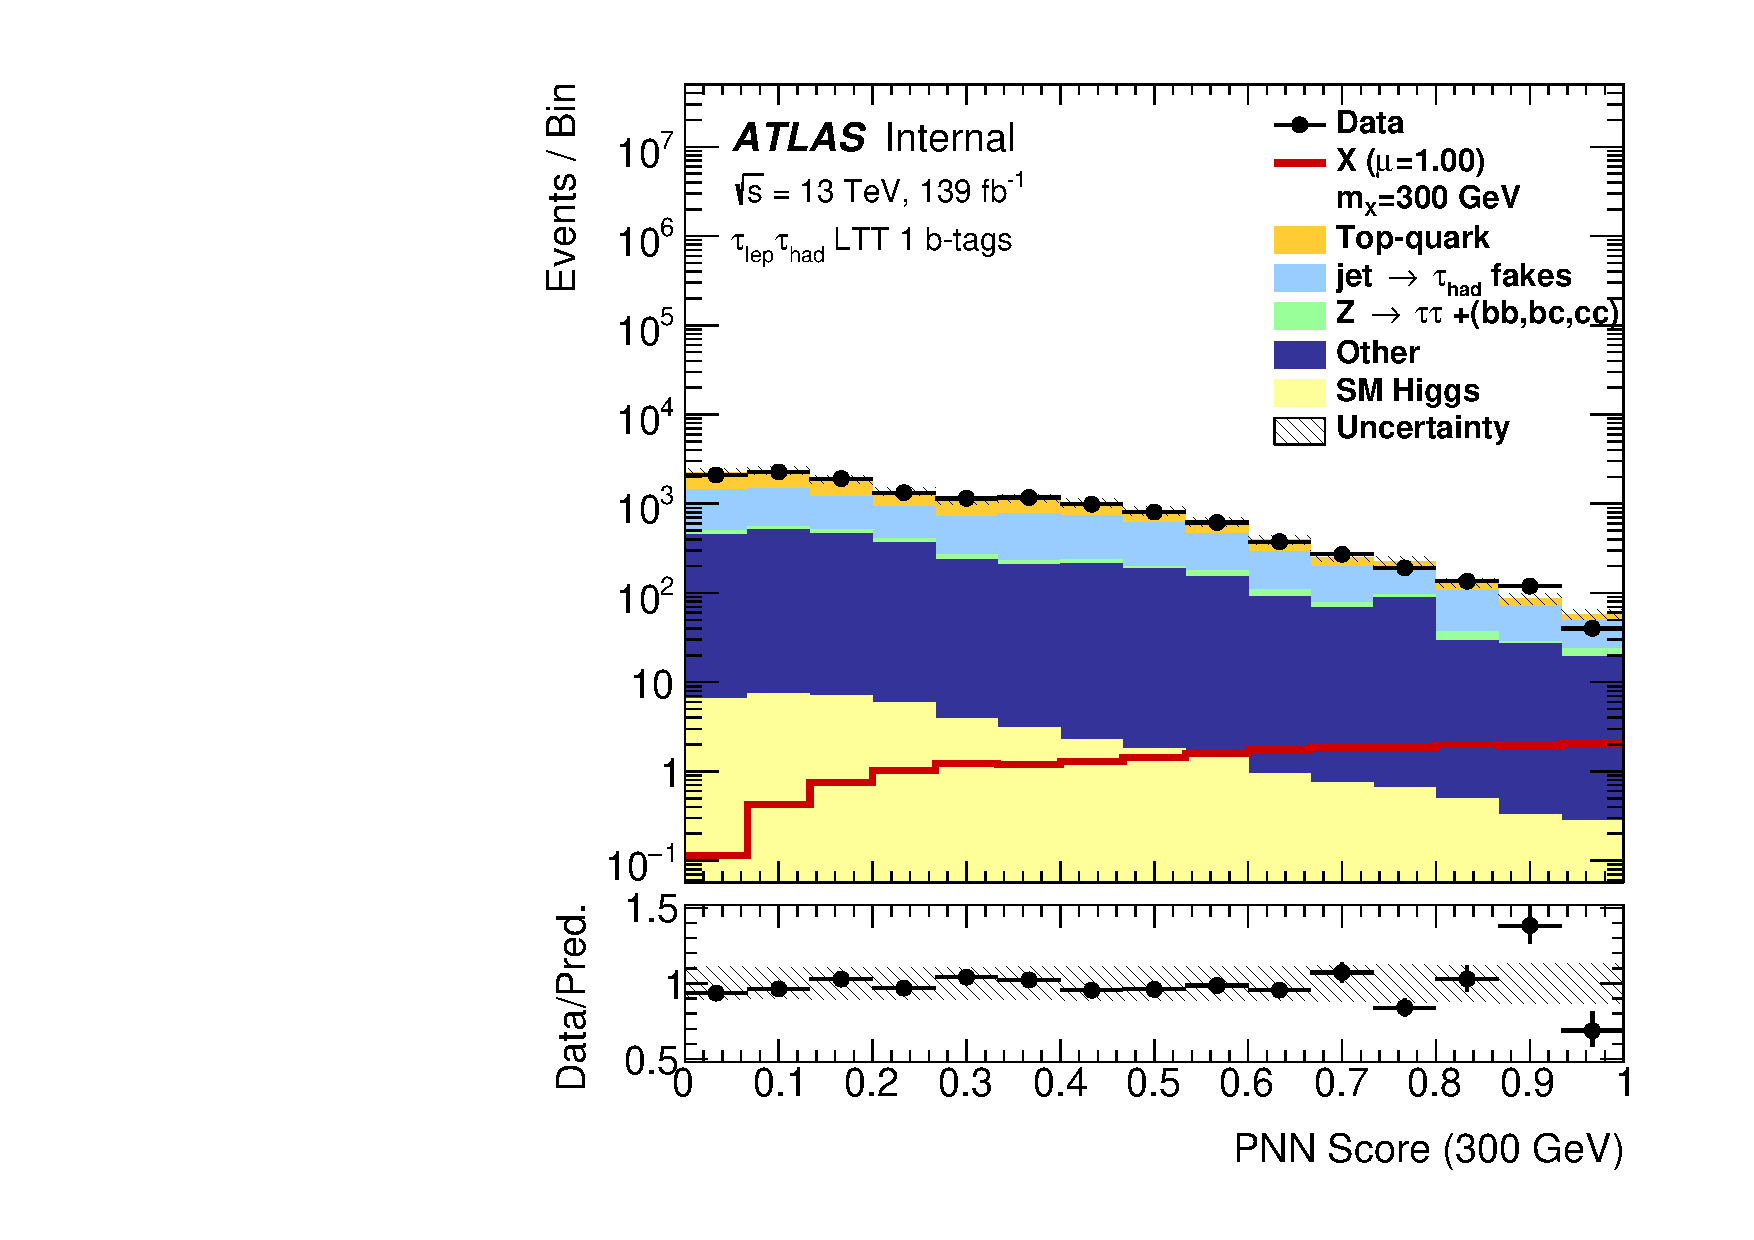
\includegraphics[width=.32\textwidth]{DiHiggs/plots/MVA/LTT/Region_BMin0_incJet1_dist300_J2_D2HDMPNN_T1_SpcTauLH_Y2015_LTT1_L1_Prefitlog.pdf}
    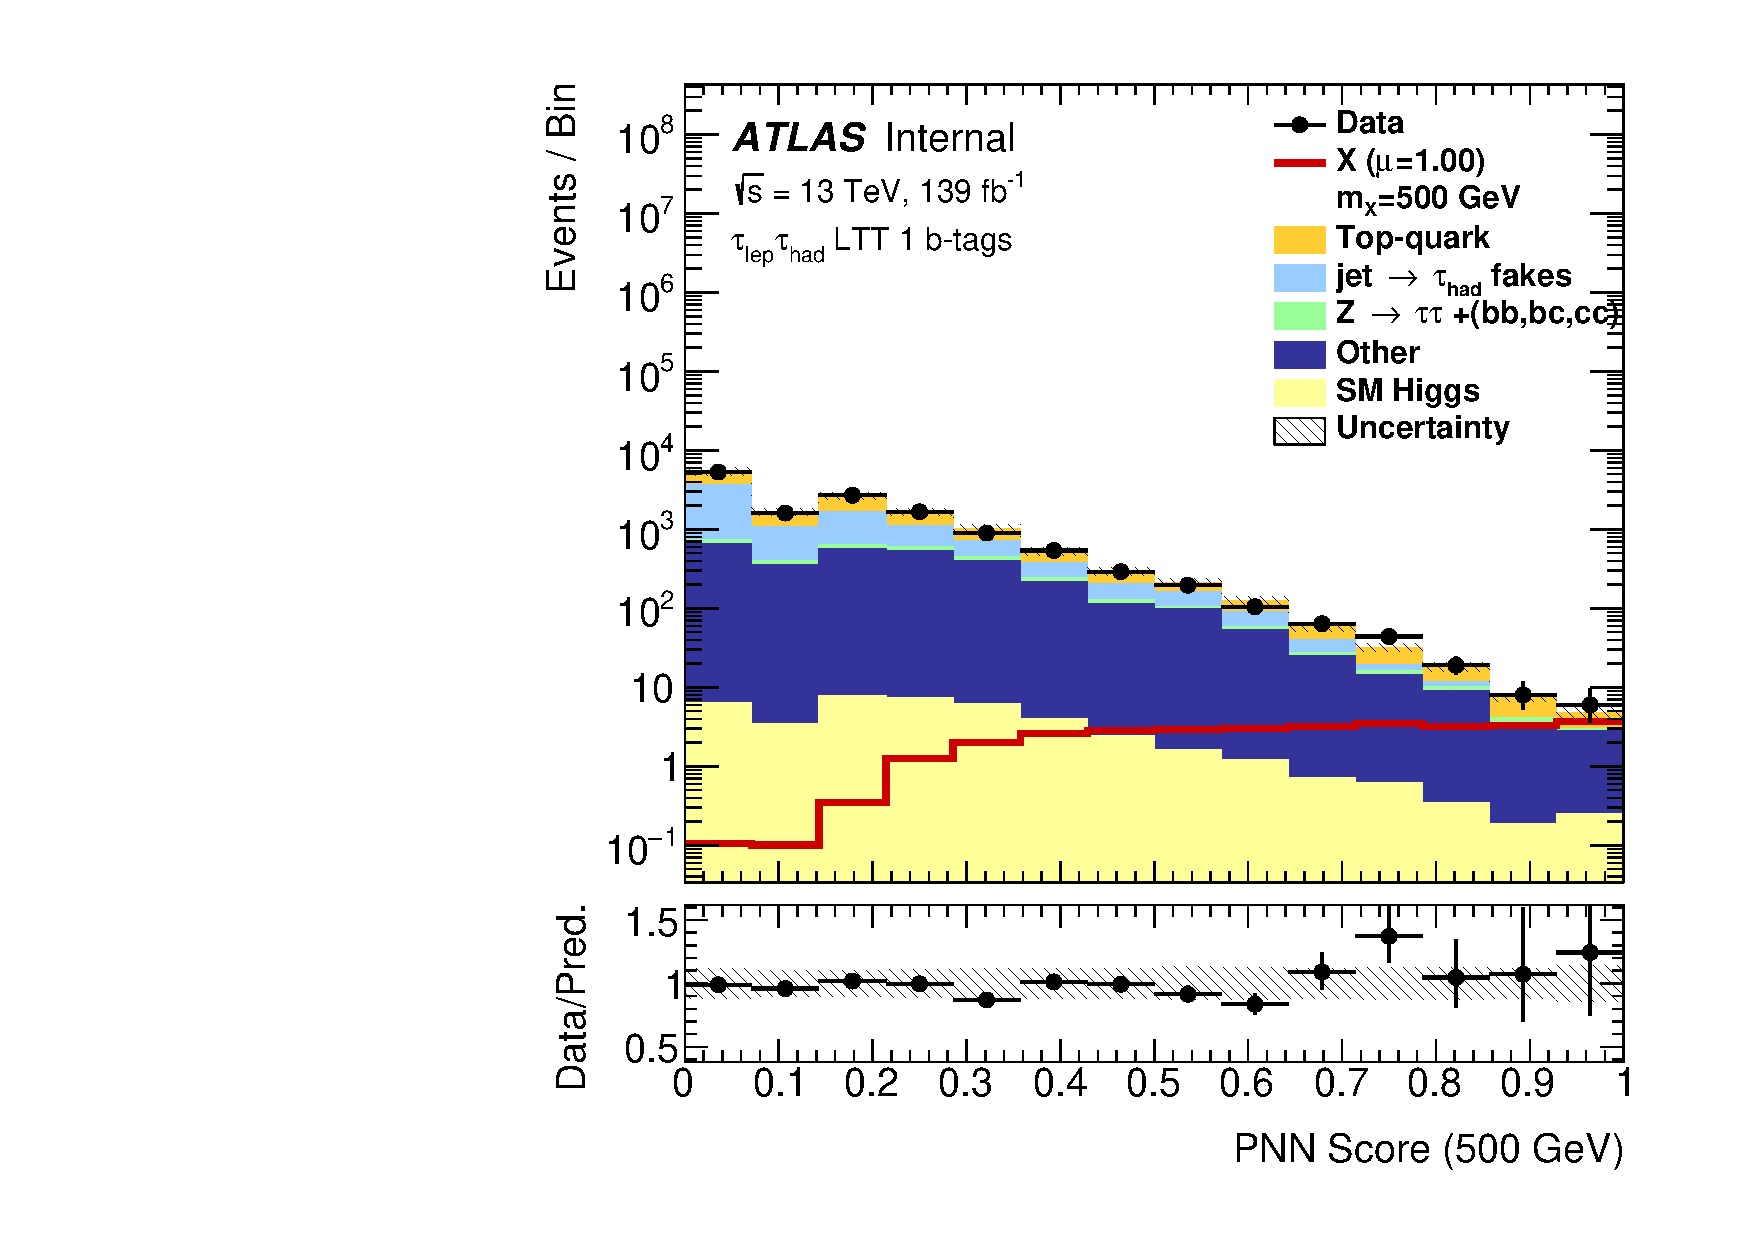
\includegraphics[width=.32\textwidth]{DiHiggs/plots/MVA/LTT/Region_BMin0_incJet1_dist500_J2_D2HDMPNN_T1_SpcTauLH_Y2015_LTT1_L1_Prefitlog.pdf}
    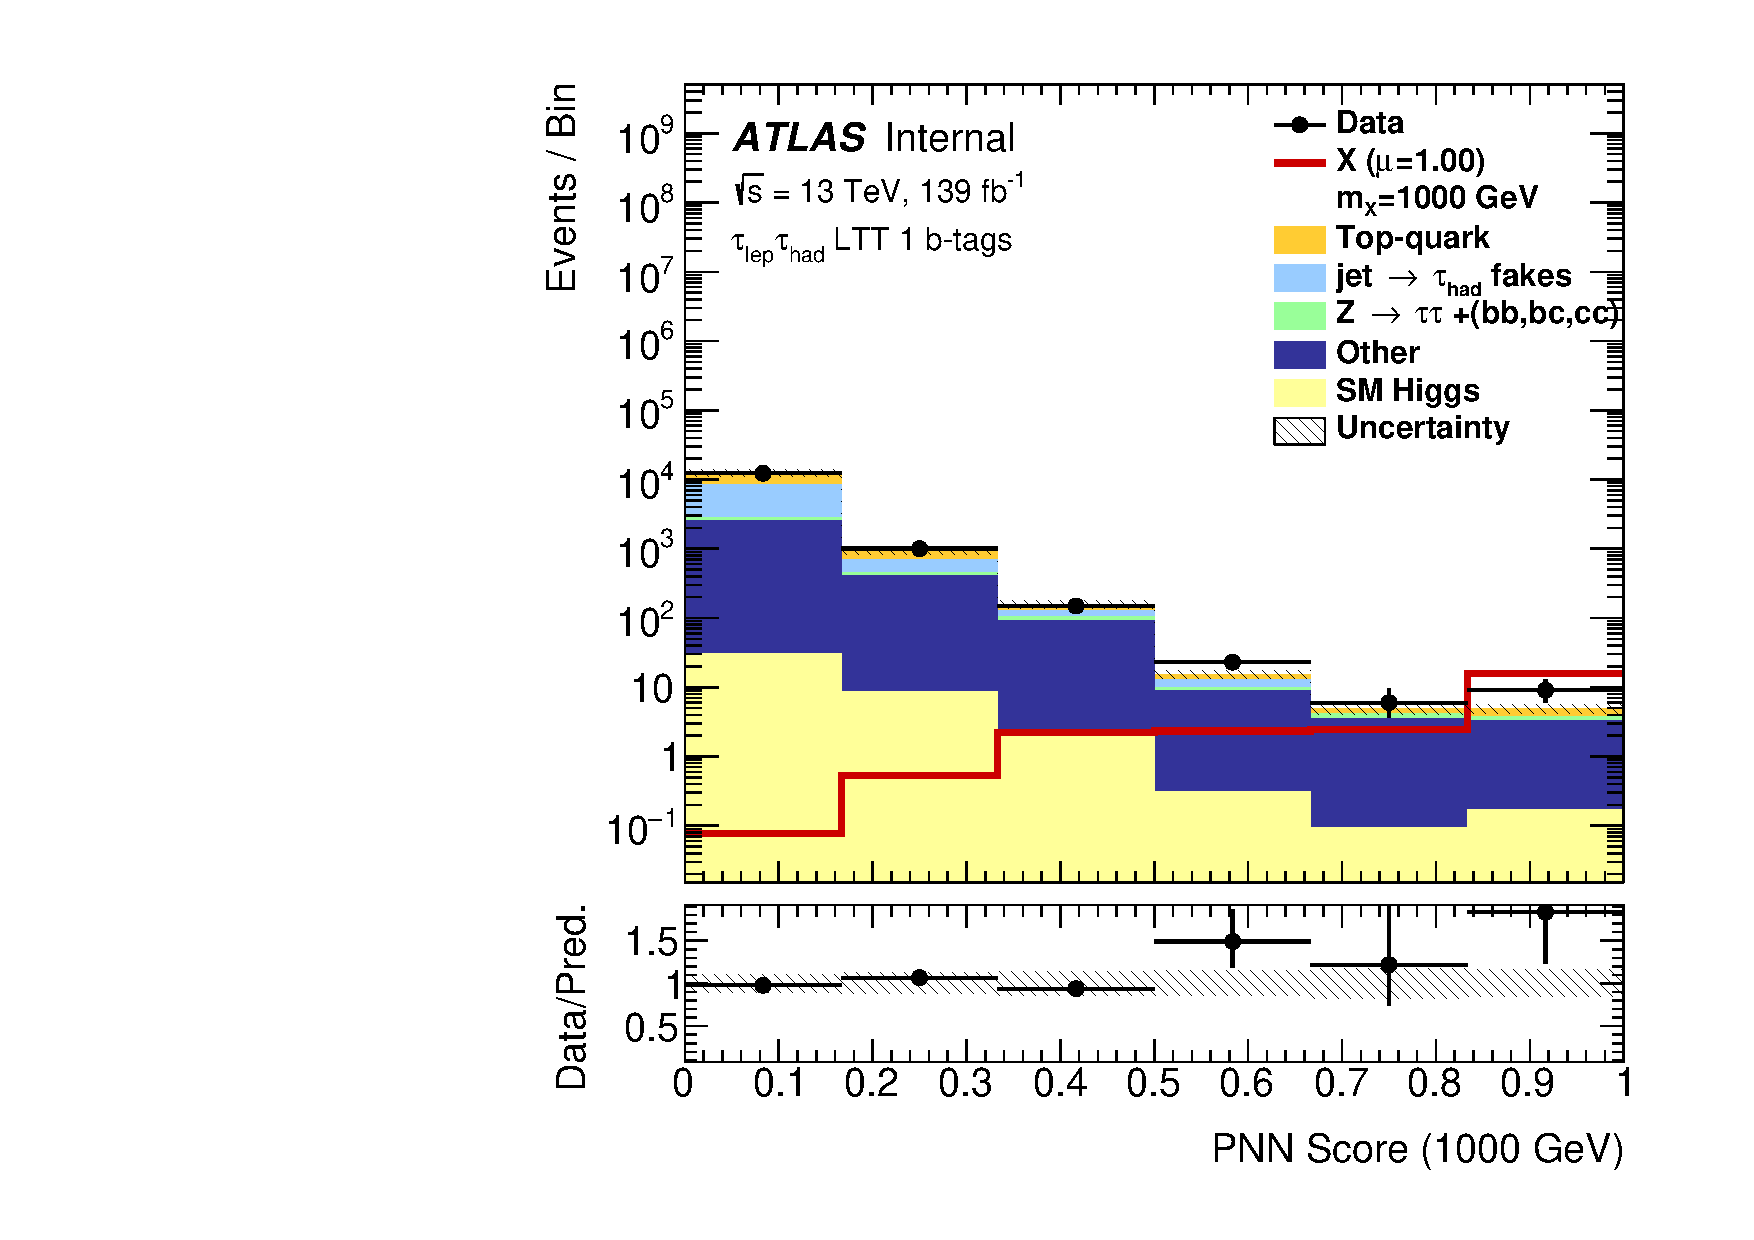
\includegraphics[width=.32\textwidth]{DiHiggs/plots/MVA/LTT/Region_BMin0_incJet1_dist1000_J2_D2HDMPNN_T1_SpcTauLH_Y2015_LTT1_L1_Prefitlog.pdf} \\
    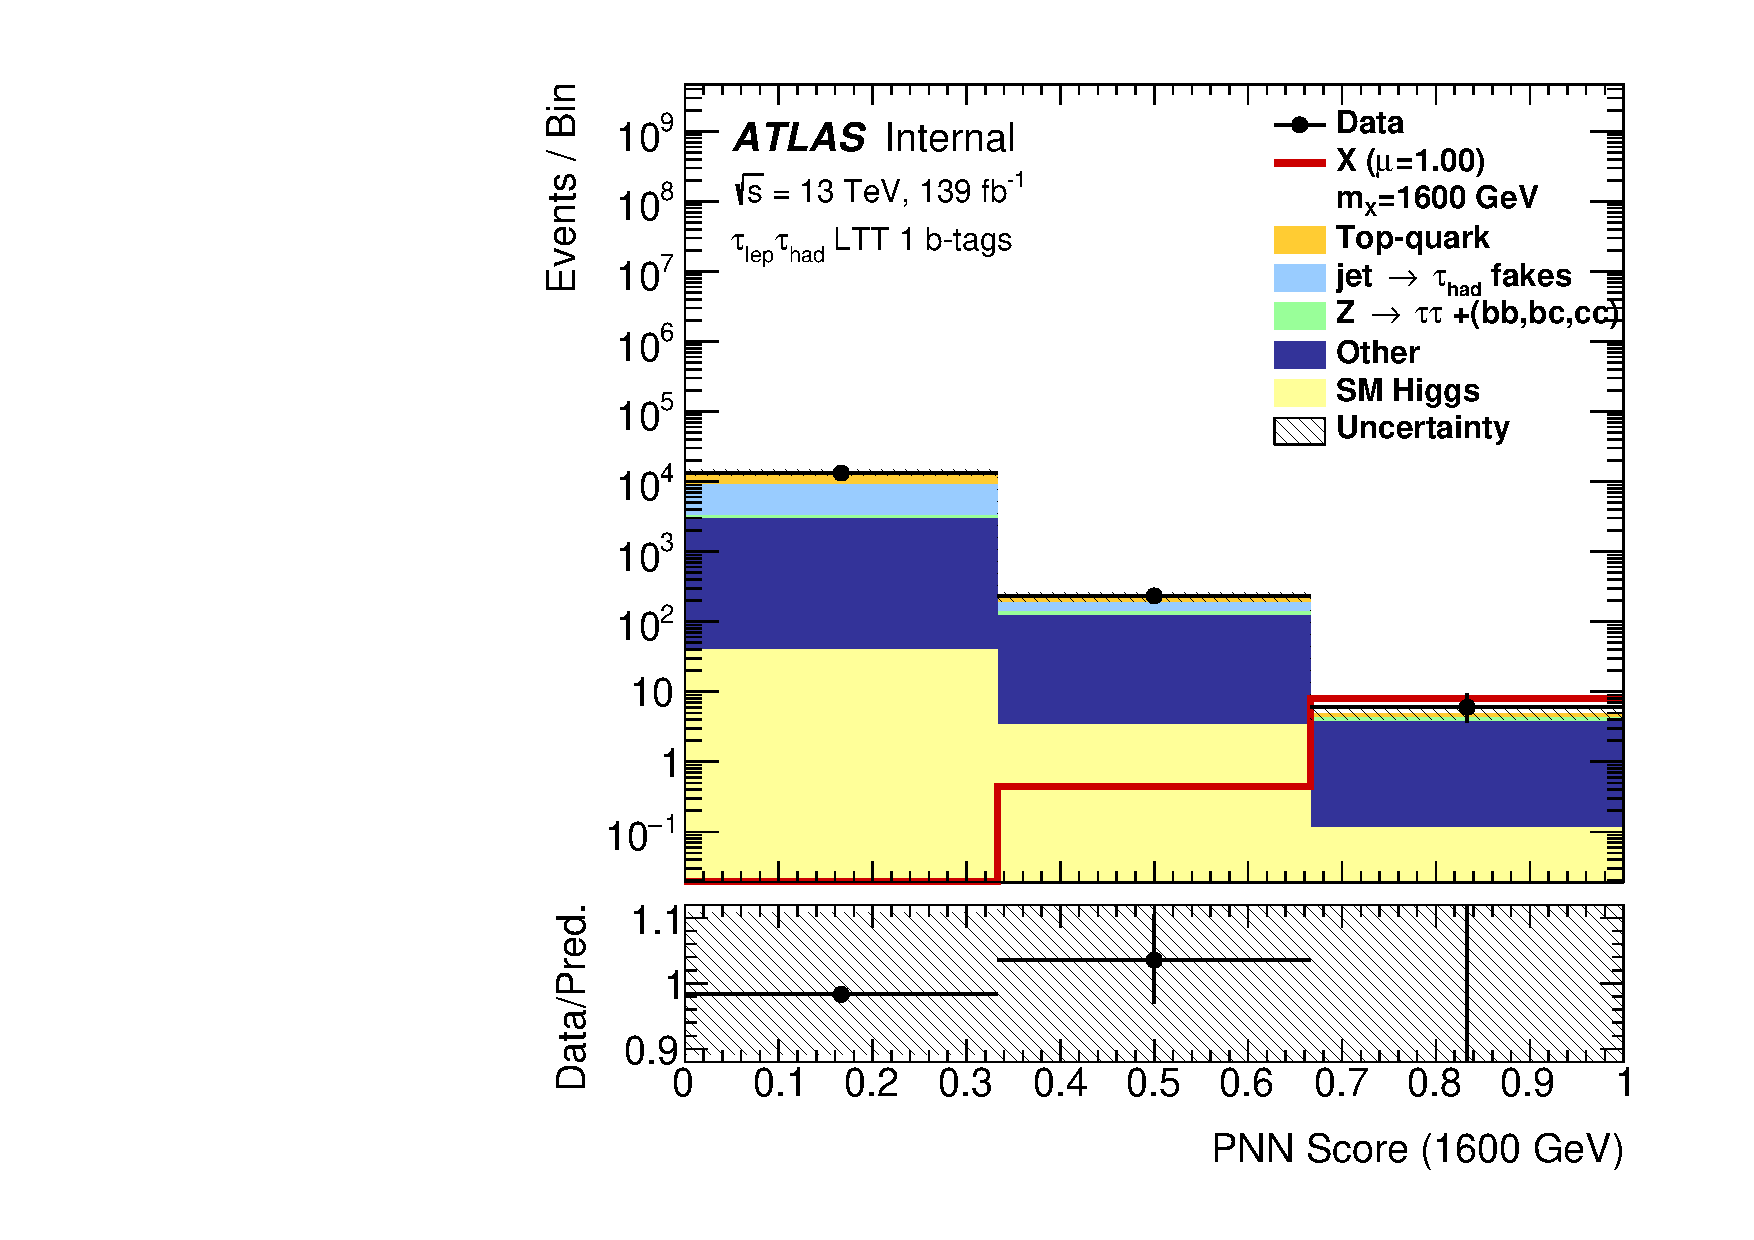
\includegraphics[width=.32\textwidth]{DiHiggs/plots/MVA/LTT/Region_BMin0_incJet1_dist1600_J2_D2HDMPNN_T1_SpcTauLH_Y2015_LTT1_L1_Prefitlog.pdf}
    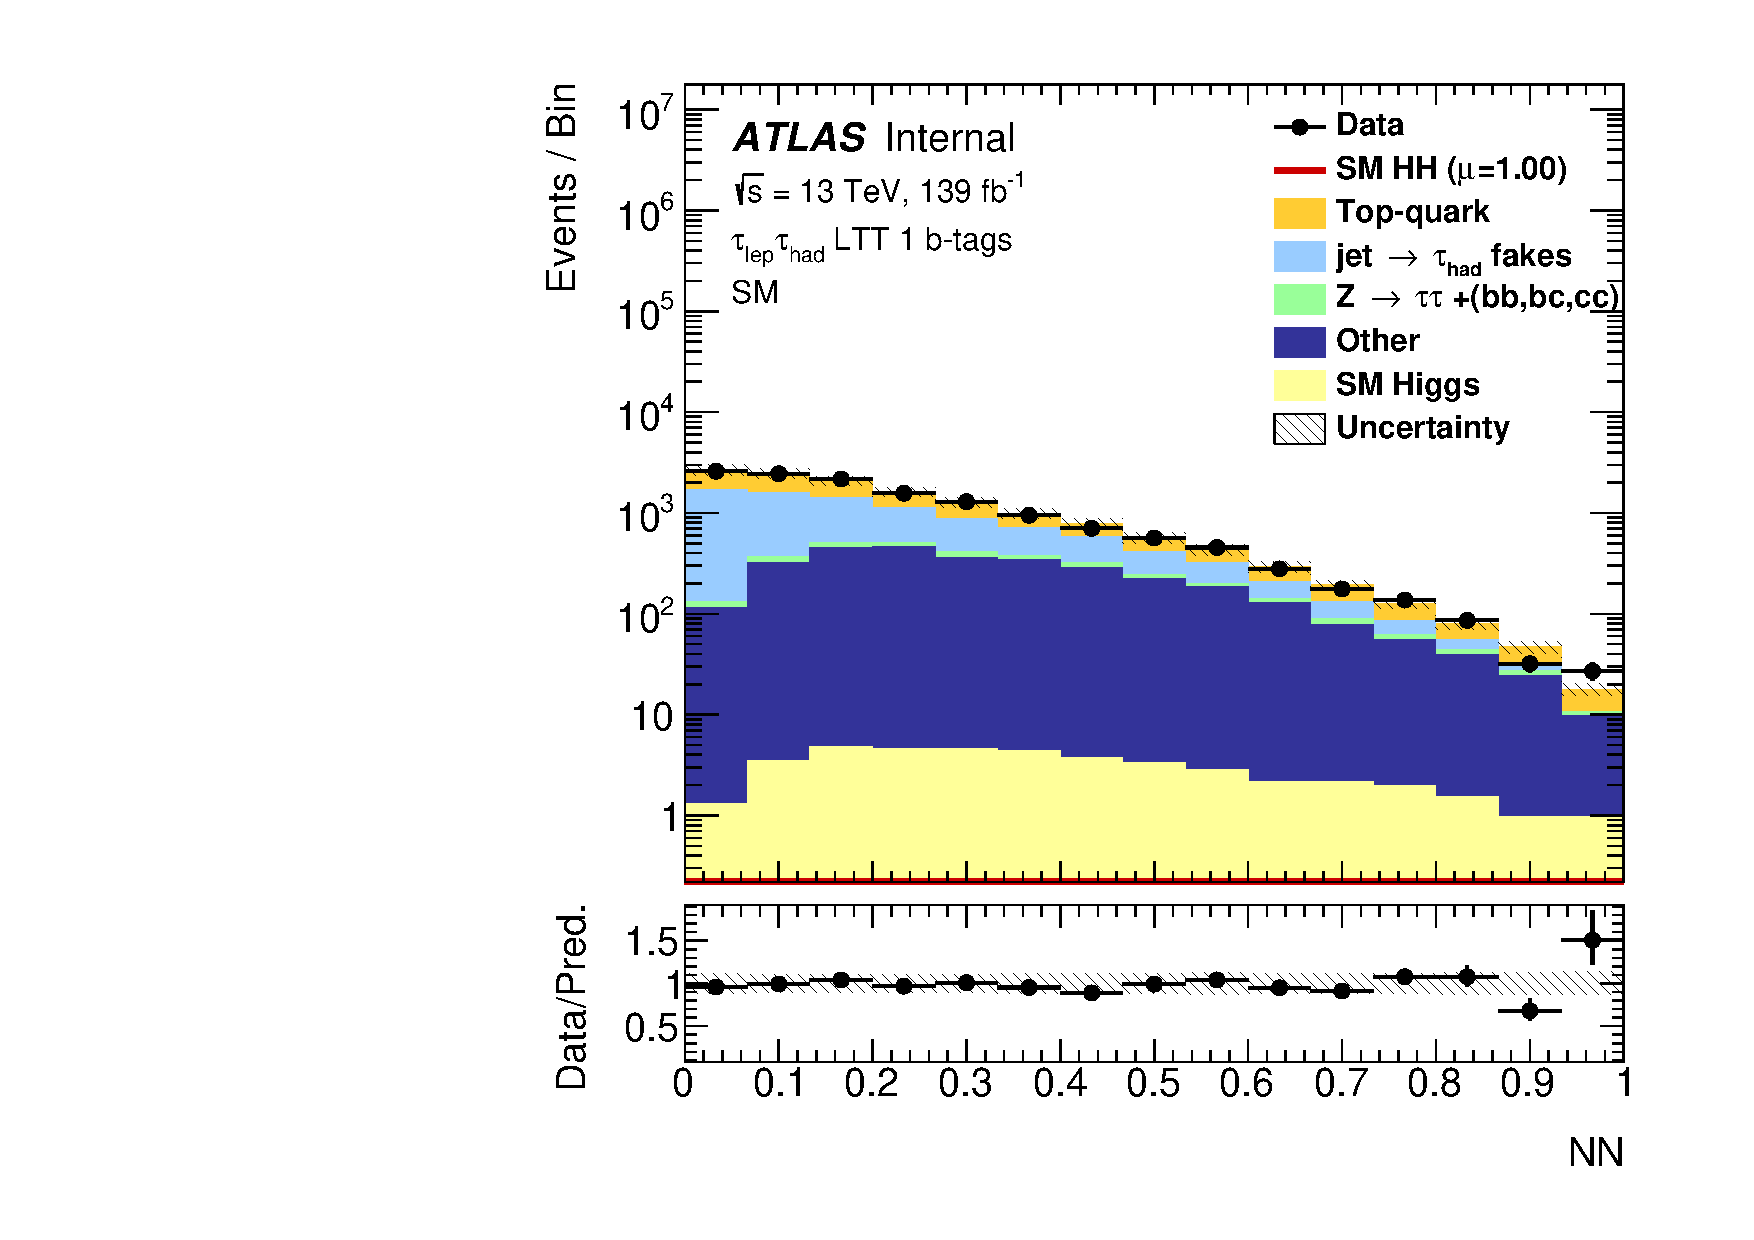
\includegraphics[width=.32\textwidth]{DiHiggs/plots/MVA/LTT/Region_BMin0_incJet1_distNN_J2_DSM_T1_SpcTauLH_Y2015_LTT1_L1_Prefitlog.pdf}
    \caption{Pre-fit PNN score distributions for the $300, 500, 1000, 1600$ 
    GeV mass points and non-resonant NN in the di-Higgs $bb\lephad$ SLT (top two rows) and LTT (bottom two rows) 1tag control regions.}
    \label{fig:lephadmvaCRoutput}
    \end{figure}


  \begin{table}
    \centering
    \footnotesize
    \begin{tabular}{|c|c|c|c|c|}
    \hline
    \multicolumn{5}{|c|}{Last bin}\\
    \hline
    Process & Last bin SM & Last bin 300 GeV & Last bin 500 GeV & Last bin 1000 GeV\\
    \hline
    ttbar &  $0.46 \pm 0.22$ &  $30.9 \pm 2$ &  $1.3 \pm 0.4$ &  $0.68 \pm 0.28$ \\
    Fake &  $1.2 \pm 0.7$ &  $16.7 \pm 2.4$ &  $1.1 \pm 0.6$ &  $0.8 \pm 0.6$ \\
    Stop &  $0.93 \pm 0.35$ &  $3 \pm 0.6$ &  $0.96 \pm 0.35$ &  $0.9 \pm 0.34$ \\
    ZHF &  $1.32 \pm 0.26$ &  $8.6 \pm 3.2$ &  $1.36 \pm 0.28$ &  $1.94 \pm 0.25$ \\
    ZLF &  $0.04 \pm 0.025$ &  $-0.25 \pm 0.25$ &  $0.029 \pm 0.029$ &  $0.27 \pm 0.18$ \\
    WHbb &  $0.0005 \pm 0.00035$ & 0 &  $0.0021 \pm 0.0012$ &  $0.0033 \pm 0.0013$ \\
    WHtautau & 0 & 0 &  $0.006 \pm 0.006$ & 0 \\
    qqZHbb &  $0.278 \pm 0.006$ &  $0.048 \pm 0.008$ &  $0.078 \pm 0.004$ &  $0.393 \pm 0.007$ \\
    ggZHbb &  $0.054 \pm 0.004$ &  $0.0008 \pm 0.0005$ &  $0.09 \pm 0.05$ &  $0.0342 \pm 0.0034$ \\
    qqZHtautau &  $0.28 \pm 0.04$ &  $0.059 \pm 0.016$ &  $0.084 \pm 0.023$ &  $0.158 \pm 0.028$ \\
    ggZHtautau &  $0.052 \pm 0.014$ &  $0.00016 \pm 0.00016$ &  $0.061 \pm 0.015$ &  $0.032 \pm 0.011$ \\
    ggFHtautau &  $0.25 \pm 0.05$ & 0 &  $0.111 \pm 0.034$ &  $0.15 \pm 0.04$ \\
    VBFHtautau &  $0.0047 \pm 0.0028$ &  $0.0025 \pm 0.0019$ &  $0.0018 \pm 0.0018$ &  $0.011 \pm 0.004$ \\
    ttH &  $0.221 \pm 0.019$ &  $0.09 \pm 0.012$ &  $0.166 \pm 0.016$ &  $0.082 \pm 0.012$ \\
    Wjets & 0 & 0 & 0 & 0 \\
    Diboson &  $0.2 \pm 0.09$ &  $0.24 \pm 0.09$ &  $0.15 \pm 0.09$ &  $0.53 \pm 0.13$ \\
    DY & 0 & 0 & 0 & 0 \\
     \hline 
    signal ggF &  $0.764 \pm 0.007$ &  $8.03 \pm 0.19$ &  $61.2 \pm 0.8$ &  $342.5 \pm 2.1$ \\
    signal VBF &  $0.00743 \pm 0.00024$  & NA  & NA  & NA  \\  
    \hline
    \multicolumn{5}{|c|}{Second-to-last bin}\\
    \hline
    Process & Last-1 bin SM & Last-1 bin 300 GeV & Last-1 bin 500 GeV & Last-1 bin 1000 GeV\\
      \hline
      ttbar &  $4.5 \pm 0.8$ &  $61.4 \pm 2.9$ &  $3.1 \pm 0.6$ &  $0.82 \pm 0.34$ \\
      Fake &  $1.9 \pm 0.8$ &  $25.4 \pm 3.2$ &  $0.8 \pm 0.6$ &  $1.4 \pm 0.8$ \\
      Stop &  $2.4 \pm 0.6$ &  $3 \pm 0.6$ &  $1.3 \pm 0.4$ &  $1.05 \pm 0.34$ \\
      ZHF &  $4 \pm 0.6$ &  $13 \pm 4$ &  $1.44 \pm 0.33$ &  $2.64 \pm 0.32$ \\
      ZLF &  $0.3 \pm 0.12$ &  $0.29 \pm 0.27$ &  $0.11 \pm 0.08$ &  $-0.03 \pm 0.08$ \\
      WHbb &  $0.0044 \pm 0.0015$ & 0 &  $0.0026 \pm 0.0015$ &  $0.0029 \pm 0.001$ \\
      WHtautau &  $0.013 \pm 0.009$ & 0 & 0 & 0 \\
      qqZHbb &  $0.448 \pm 0.008$ &  $0.086 \pm 0.01$ &  $0.075 \pm 0.004$ &  $0.232 \pm 0.005$ \\
      ggZHbb &  $0.16 \pm 0.05$ &  $0.0022 \pm 0.0008$ &  $0.0331 \pm 0.0034$ &  $0.06 \pm 0.04$ \\
      qqZHtautau &  $0.44 \pm 0.05$ &  $0.07 \pm 0.018$ &  $0.099 \pm 0.021$ &  $0.14 \pm 0.026$ \\
      ggZHtautau &  $0.126 \pm 0.022$ & 0 &  $0.059 \pm 0.015$ &  $0.017 \pm 0.008$ \\
      ggFHtautau &  $0.25 \pm 0.05$ &  $0.069 \pm 0.029$ &  $0.093 \pm 0.034$ &  $0.17 \pm 0.04$ \\
      VBFHtautau &  $0.012 \pm 0.005$ &  $0.009 \pm 0.004$ &  $0.0031 \pm 0.0022$ &  $0.01 \pm 0.004$ \\
      ttH &  $0.27 \pm 0.021$ &  $0.11 \pm 0.012$ &  $0.128 \pm 0.014$ &  $0.07 \pm 0.01$ \\
      Wjets & 0 & 0 & 0 & 0 \\
      Diboson &  $0.56 \pm 0.17$ &  $0.55 \pm 0.2$ &  $0.12 \pm 0.07$ &  $0.82 \pm 0.18$ \\
      DY & 0 & 0 & 0 & 0 \\
      \hline 
      signal ggF &  $0.599 \pm 0.006$ &  $7.53 \pm 0.18$ &  $21 \pm 0.5$ &  $42 \pm 0.7$ \\
      signal VBF &  $0.00869 \pm 0.00027$ & NA  & NA  & NA  \\    
      \hline
      \multicolumn{5}{|c|}{Third-to-last bin}\\
      \hline
      Process & Last-2 bin SM & Last-2 bin 300 GeV & Last-2 bin 500 GeV & Last-2 bin 1000 GeV\\
      \hline
      ttbar &  $9.1 \pm 1.1$ &  $88 \pm 3.4$ &  $5.2 \pm 0.9$ &  $209 \pm 5$ \\ 
      Fake &  $4.7 \pm 1.5$ &  $44 \pm 4$ &  $3.6 \pm 1.2$ &  $395 \pm 13$ \\ 
      Stop &  $5.3 \pm 0.8$ &  $4.3 \pm 0.7$ &  $1.2 \pm 0.4$ &  $104 \pm 4$ \\ 
      ZHF &  $7.1 \pm 0.7$ &  $11 \pm 4$ &  $3.3 \pm 0.7$ &  $212 \pm 6$ \\ 
      ZLF &  $0.54 \pm 0.28$ &  $0.9 \pm 0.7$ &  $0.04 \pm 0.11$ &  $21.9 \pm 2.9$ \\ 
      WHbb &  $0.021 \pm 0.004$ &  $0.013 \pm 0.008$ &  $0.0053 \pm 0.002$ &  $0.511 \pm 0.018$ \\ 
      WHtautau & 0 & 0 &  $0.005 \pm 0.005$ &  $0.101 \pm 0.029$ \\ 
      qqZHbb &  $0.677 \pm 0.011$ &  $0.123 \pm 0.012$ &  $0.121 \pm 0.006$ &  $3.355 \pm 0.022$ \\ 
      ggZHbb &  $0.24 \pm 0.06$ &  $0.0024 \pm 0.0009$ &  $0.043 \pm 0.004$ &  $1.31 \pm 0.11$ \\ 
      qqZHtautau &  $0.45 \pm 0.05$ &  $0.063 \pm 0.018$ &  $0.159 \pm 0.028$ &  $1.71 \pm 0.09$ \\ 
      ggZHtautau &  $0.161 \pm 0.024$ & 0 &  $0.059 \pm 0.015$ &  $0.57 \pm 0.05$ \\ 
      ggFHtautau &  $0.41 \pm 0.07$ &  $0.089 \pm 0.033$ &  $0.092 \pm 0.031$ &  $4.23 \pm 0.22$ \\ 
      VBFHtautau &  $0.033 \pm 0.008$ &  $0.009 \pm 0.004$ &  $0.01 \pm 0.004$ &  $0.402 \pm 0.026$ \\ 
      ttH &  $0.482 \pm 0.028$ &  $0.159 \pm 0.015$ &  $0.188 \pm 0.017$ &  $4.45 \pm 0.08$ \\ 
      Wjets &  $0.08 \pm 0.08$ &  $0.07 \pm 0.07$ & 0 &  $6 \pm 0.9$ \\ 
      Diboson &  $1.03 \pm 0.19$ &  $0.95 \pm 0.22$ &  $0.26 \pm 0.08$ &  $22.2 \pm 1.5$ \\ 
      DY & 0 & 0 & 0 &  $0.7 \pm 0.4$ \\ 
      \hline  
      signal ggF &  $0.596 \pm 0.006$ &  $7.36 \pm 0.18$ &  $20.6 \pm 0.5$ &  $40.5 \pm 0.7$ \\ 
      signal VBF &  $0.00997 \pm 0.00029$  & NA  & NA  & NA  \\ 
      \hline
    \end{tabular}
    \caption{Pre-fit event yields in the last, second-to-last and
    third-to-last MVA bin of the di-Higgs \lephad SLT channel.}
    \label{tab:yields_LastMVABin_LepHad_SLT}
    \end{table}
   
  
  
  
  \begin{table}
    \centering
    \footnotesize
    \begin{tabular}{|c|c|c|c|c|}
    \hline
    \multicolumn{5}{|c|}{Last bin}\\
    \hline
    Process & Last bin SM & Last bin 300 GeV & Last bin 500 GeV & Last bin 1000 GeV\\
    \hline
    ttbar &  $0.76 \pm 0.31$ &  $5 \pm 0.8$ &  $2.3 \pm 0.6$ &  $0.57 \pm 0.29$  \\
    Fake &  $2.6 \pm 1.4$ &  $3.7 \pm 1.7$ &  $1 \pm 0.8$ &  $0.9 \pm 0.9$  \\
    Stop &  $0.32 \pm 0.19$ &  $0.14 \pm 0.14$ &  $0.17 \pm 0.12$ &  $0.47 \pm 0.25$  \\
    ZHF &  $1.03 \pm 0.23$ &  $3.3 \pm 2.2$ &  $1.3 \pm 0.4$ &  $2.1 \pm 0.5$  \\
    ZLF &  $0.07 \pm 0.07$ & 0 &  $0.05 \pm 0.09$ &  $0.52 \pm 0.24$  \\
    WHbb &  $0.0013 \pm 0.0009$ & 0 & 0 &  $0.004 \pm 0.004$  \\
    WHtautau & 0 & 0 & 0 & 0  \\
    qqZHbb &  $0.0656 \pm 0.0032$ &  $0.0073 \pm 0.0028$ &  $0.0416 \pm 0.0027$ &  $0.0785 \pm 0.0032$  \\
    ggZHbb &  $0.0191 \pm 0.0026$ &  $0.0004 \pm 0.0004$ &  $0.0182 \pm 0.0024$ &  $0.0063 \pm 0.0014$  \\
    qqZHtautau &  $0.065 \pm 0.018$ &  $0.019 \pm 0.01$ &  $0.051 \pm 0.016$ &  $0.052 \pm 0.018$  \\
    ggZHtautau &  $0.02 \pm 0.009$ & 0 &  $0.022 \pm 0.009$ & 0  \\
    ggFHtautau &  $0.076 \pm 0.034$ & 0 &  $0.076 \pm 0.03$ &  $0.11 \pm 0.04$  \\
    VBFHtautau &  $0.005 \pm 0.0029$ & 0 &  $0.0018 \pm 0.0018$ &  $0.0035 \pm 0.0025$  \\
    ttH &  $0.044 \pm 0.008$ &  $0.014 \pm 0.005$ &  $0.065 \pm 0.01$ &  $0.031 \pm 0.007$  \\
    Wjets & 0 & 0 & 0 & 0  \\
    Diboson &  $-0.01 \pm 0.05$ &  $-0.05 \pm 0.04$ &  $0.03 \pm 0.04$ &  $0.44 \pm 0.14$  \\
    DY & 0 & 0 & 0 & 0  \\
    \hline   
   signal ggF &  $0.1977 \pm 0.0035$ &  $2.61 \pm 0.11$ &  $20.8 \pm 0.5$ &  $45.1 \pm 0.8$  \\
   signal VBF &  $0.00344 \pm 0.00017$ & NA  & NA  & NA  \\
    \hline
    \multicolumn{5}{|c|}{Second-to-last bin}\\
    \hline
    Process & Last-1 bin SM & Last-1 bin 300 GeV & Last-1 bin 500 GeV & Last-1 bin 1000 GeV\\
      \hline
      ttbar &  $3.8 \pm 0.7$ &  $8.5 \pm 1.1$ &  $2.5 \pm 0.6$ &  $108 \pm 4$ \\
      Fake &  $2 \pm 1.4$ &  $1.4 \pm 1.1$ &  $1.7 \pm 1.2$ &  $84 \pm 9$ \\
      Stop &  $0.37 \pm 0.21$ &  $0.45 \pm 0.24$ &  $0.08 \pm 0.08$ &  $18 \pm 1.7$ \\
      ZHF &  $1.6 \pm 0.4$ &  $2.5 \pm 1.1$ &  $0.82 \pm 0.19$ &  $86.4 \pm 3.4$ \\
      ZLF &  $0.15 \pm 0.1$ &  $0.07 \pm 0.07$ & 0 &  $11 \pm 4$ \\
      WHbb & 0 &  $0.0027 \pm 0.0027$ &  $0.0016 \pm 0.0011$ &  $0.0074 \pm 0.002$ \\
      WHtautau & 0 & 0 & 0 &  $0.047 \pm 0.021$ \\
      qqZHbb &  $0.083 \pm 0.004$ &  $0.022 \pm 0.005$ &  $0.0384 \pm 0.0033$ &  $0.826 \pm 0.013$ \\
      ggZHbb &  $0.0262 \pm 0.0029$ &  $0.00022 \pm 0.00016$ &  $0.0154 \pm 0.0023$ &  $0.44 \pm 0.06$ \\
      qqZHtautau &  $0.088 \pm 0.021$ &  $0.011 \pm 0.008$ &  $0.06 \pm 0.018$ &  $0.57 \pm 0.05$ \\
      ggZHtautau &  $0.027 \pm 0.01$ & 0 &  $0.028 \pm 0.01$ &  $0.212 \pm 0.028$ \\
      ggFHtautau &  $0.094 \pm 0.032$ &  $0.015 \pm 0.011$ &  $0.022 \pm 0.015$ &  $1.48 \pm 0.14$ \\
      VBFHtautau &  $0.005 \pm 0.0029$ &  $0.0025 \pm 0.0024$ &  $0.0043 \pm 0.0027$ &  $0.12 \pm 0.014$ \\
      ttH &  $0.062 \pm 0.01$ &  $0.02 \pm 0.005$ &  $0.046 \pm 0.009$ &  $1.45 \pm 0.05$ \\
      Wjets & 0 & 0 & 0 &  $0.83 \pm 0.31$ \\
      Diboson &  $0.14 \pm 0.08$ &  $0.1 \pm 0.09$ &  $0 \pm 0.04$ &  $3.7 \pm 0.4$ \\
      DY & 0 & 0 &  $0.15 \pm 0.15$ &  $0.15 \pm 0.15$ \\
       \hline 
      signal ggF&  $0.1402 \pm 0.0028$ &  $2.72 \pm 0.11$ &  $5.87 \pm 0.25$ &  $2.28 \pm 0.17$ \\
      signal VBF&  $0.00294 \pm 0.00016$ & NA  & NA  & NA  \\
      \hline
      \multicolumn{5}{|c|}{Third-to-last bin}\\
      \hline
      Process & Last-2 bin SM & Last-2 bin 300 GeV & Last-2 bin 500 GeV & Last-2 bin 1000 GeV\\
      \hline
      ttbar &  $6.3 \pm 0.9$ &  $9.7 \pm 1.2$ &  $3.4 \pm 0.7$ &  $4104 \pm 24$ \\
      Fake &  $1.4 \pm 1.3$ &  $6.6 \pm 2.4$ &  $2.4 \pm 1.3$ &  $2060 \pm 40$ \\
      Stop &  $0.85 \pm 0.34$ &  $0.3 \pm 0.21$ &  $0.47 \pm 0.25$ &  $179 \pm 5$ \\
      ZHF &  $4.8 \pm 0.9$ &  $2.6 \pm 1.1$ &  $2.1 \pm 0.4$ &  $368 \pm 14$ \\
      ZLF &  $0.18 \pm 0.09$ &  $0.25 \pm 0.2$ &  $0.05 \pm 0.04$ &  $37 \pm 9$ \\
      WHbb &  $0.0012 \pm 0.0008$ & 0 &  $0.001 \pm 0.0007$ &  $0.162 \pm 0.026$ \\
      WHtautau & 0 &  $0.006 \pm 0.006$ & 0 &  $0.131 \pm 0.033$ \\
      qqZHbb &  $0.124 \pm 0.006$ &  $0.041 \pm 0.007$ &  $0.0457 \pm 0.0032$ &  $2.95 \pm 0.05$ \\
      ggZHbb &  $0.0323 \pm 0.0032$ &  $0.0013 \pm 0.0006$ &  $0.0221 \pm 0.0026$ &  $1.01 \pm 0.13$ \\
      qqZHtautau &  $0.129 \pm 0.026$ &  $0.015 \pm 0.009$ &  $0.052 \pm 0.016$ &  $1.56 \pm 0.09$ \\
      ggZHtautau &  $0.039 \pm 0.012$ &  $0.004 \pm 0.004$ &  $0.028 \pm 0.01$ &  $0.53 \pm 0.04$ \\
      ggFHtautau &  $0.098 \pm 0.029$ &  $0.005 \pm 0.005$ &  $0.085 \pm 0.035$ &  $2.98 \pm 0.2$ \\
      VBFHtautau &  $0.014 \pm 0.005$ &  $0.0019 \pm 0.0019$ &  $0.0033 \pm 0.0023$ &  $0.248 \pm 0.02$ \\
      ttH &  $0.111 \pm 0.013$ &  $0.024 \pm 0.006$ &  $0.043 \pm 0.008$ &  $9.52 \pm 0.11$ \\
      Wjets & 0 & 0 & 0 &  $3.2 \pm 1$ \\
      Diboson &  $0.18 \pm 0.08$ &  $0 \pm 0.08$ &  $0.09 \pm 0.07$ &  $16.3 \pm 1$ \\
      DY & 0 & 0 & 0 &  $0.68 \pm 0.29$ \\
       \hline 
      signal ggF &  $0.1382 \pm 0.0028$ &  $2.61 \pm 0.11$ &  $4.93 \pm 0.23$ &  $0.009 \pm 0.009$ \\
      signal VBF &  $0.00331 \pm 0.00017$  & NA  & NA  & NA  \\    
      \hline
    \end{tabular}
    \caption{Pre-fit event yields in the last, second-to-last and
    third-to-last MVA bin of the di-Higgs \lephad LTT channel.}
    \label{tab:yields_LastMVABin_LepHad_LTT}
    \end{table}
     